\chapter{Networking}

\epigraph{The Web as I envisaged it, we have not seen it yet.
  The future is still so much bigger than the past}{Tim Berners-Lee}

Networking has become arguably the most important use of computers in the past 10-20 years.
Most of us nowadays can't stand a place without WiFi or any connectivity, so it is crucial as programmers that you have an understanding of networking and how to program to communicate across networks.
Although it may sound complicated, POSIX has defined nice standards that make connecting to the outside world easy.
POSIX also lets you peer underneath the hood and optimize all the little parts of each connection to write highly performant programs.

As an addendum that you'll read more about in the next chapter, we will be very strict in our notation for sizes.
That means that when we refer to the SI prefixes of Kilo- Mega- etc etc, then we are always referring to a power of 10.
A kilobyte is one thousand bytes, a megabyte is a thousand kilobytes and so on.
If we need to refer to \keyword{1024} bytes, we will use the more accurate term Kibibyte. Mibibyte and Gibibyte are the analogues of Megabyte and Gigabyte respectively.
We make this distinction in order to make sure that we aren't off by 24.
The reasons for this misnomer will be explained in the filesystems chapter.

\section{The OSI Model}

The Open Source Interconnection 7 layer model (OSI Model) is a sequence of segments that define standards for both infrastructure and protocols for forms of radio communication, in our case the Internet.
The 7 layer model is as follows

\begin{enumerate}
\item Layer 1: The physical layer.
  These are the actual waves that carry the bauds across the wire.
  As an aside, bits don't cross the wire because in most mediums you can alter two characteristics of a wave -- the amplitude and the frequency -- and get more bits per clock cycle.

\item Layer 2: The link layer.
  This is how each of the agents react to certain events (error detection, noisy channels, etc).
  This is where \gls{Ethernet} and \gls{WiFi} live.

\item Layer 3: The network layer.
  This is the heart of the Internet.
  The bottom two protocols deal with communication between two different computers that are directly connected.
  This layer deals with routing packets from one endpoint to another.

\item Layer 4: The transport layer.
  This layer specifies how the slices of data are received.
  The bottom three layers make no guarantee about the order that packets are received and what happens when a packet is dropped.
  Using different protocols, this layer can.

\item Layer 5: The session layer.
  This layer makes sure that if a connection in the previous layers is dropped, a new connection in the lower layers can be established, and it looks like nothing happened to the end user.

\item Layer 6: The presentation layer.
  This layer deals with encryption, compression, and data translation.
  For example, portability between different operating systems like translating newlines to windows newlines.

\item Layer 7: The application layer.
  \gls{HTTP} and \gls{FTP} are both defined at this level.
  This is typically where we define protocols across the Internet.
  As programmers, we only go lower when we think we can create algorithms that are more suited to our needs than all of the below.

\end{enumerate}

This book won't cover networking in depth.
We will focus on some aspects of layers 3, 4, and 7 because they are essential to know if you are going to be doing something with the Internet, which at some point in your career you will be.
As for another definition, a protocol is a set of specifications put forward by the \gls{Internet Engineering Task Force} that govern how implementers of protocol have their program or circuit behave under specific circumstances.

\section{Layer 3: The Internet Protocol}

The following is a short introduction to internet protocol (IP), the primary way to send datagrams of information from one machine to another.
``IP4'', or more precisely, \gls{IPv4} is version 4 of the Internet Protocol that describes how to send \gls{packets} of information across a network from one machine to another.
Even as of 2018, IPv4 still dominates Internet traffic, but google reports that 24 countries now supply 15\% of their traffic through IPv6 \cite{internet_society_2018}.
A significant limitation of IPv4 is that source and destination addresses are limited to 32 bits.
IPv4 was designed at a time when the idea of 4 billion devices connected to the same network was unthinkable or at least not worth making the packet size larger.
\gls{IPv4 address} are written typically in a sequence of four octets delimited by periods "255.255.255.0" for example.

Each IPv4 \gls{datagram} includes a very small header - typically 20 \gls{octets}, that includes a source and destination address.
Conceptually the source and destination addresses can be split into two: a network number the upper bits and lower bits represent a particular host number on that network.

A newer packet protocol \gls{IPv6} solves many of the limitations of IPv4 like making routing tables simpler and 128 bit addresses.
However, very little web traffic is IPv6 based by comparison \cite{internet_society_2018}
We write IPv6 addresses in a sequence of eight, four hexadecimal delimiters like "1F45:0000:0000:0000:0000:0000:0000:0000".
Since that can get unruly, we can omit the zeros "1F45::". A machine can have an IPv6 address and an IPv4 address.

There are special IP Addresses.
One such in IPv4 is \keyword{127.0.0.1}, IPv6 as \keyword{0:0:0:0:0:0:0:1} or \keyword{::1} also known as localhost.
Packets sent to 127.0.0.1 will never leave the machine; the address is specified to be the same machine.
There are a lot of others that are denoted by certain octets being zeros or 255, the maximum value. You won't need to know all the terminology, just keep in mind that the actual number of IP addresses that a machine can have globally over the Internet is smaller than the number of ``raw'' addresses.
For the purposes of the class, you need to know at this layer that IP deals with routing, fragmenting, and reassembling upper level protocols. A more in-depth aside follows.

\subsection{Extra: In-depth IPv4 Specification}

The Internet Protocol deals with routing, fragmentation, and reassembly of fragments.
Datagrams are formatted as such

\begin{figure}[H]
  \centering
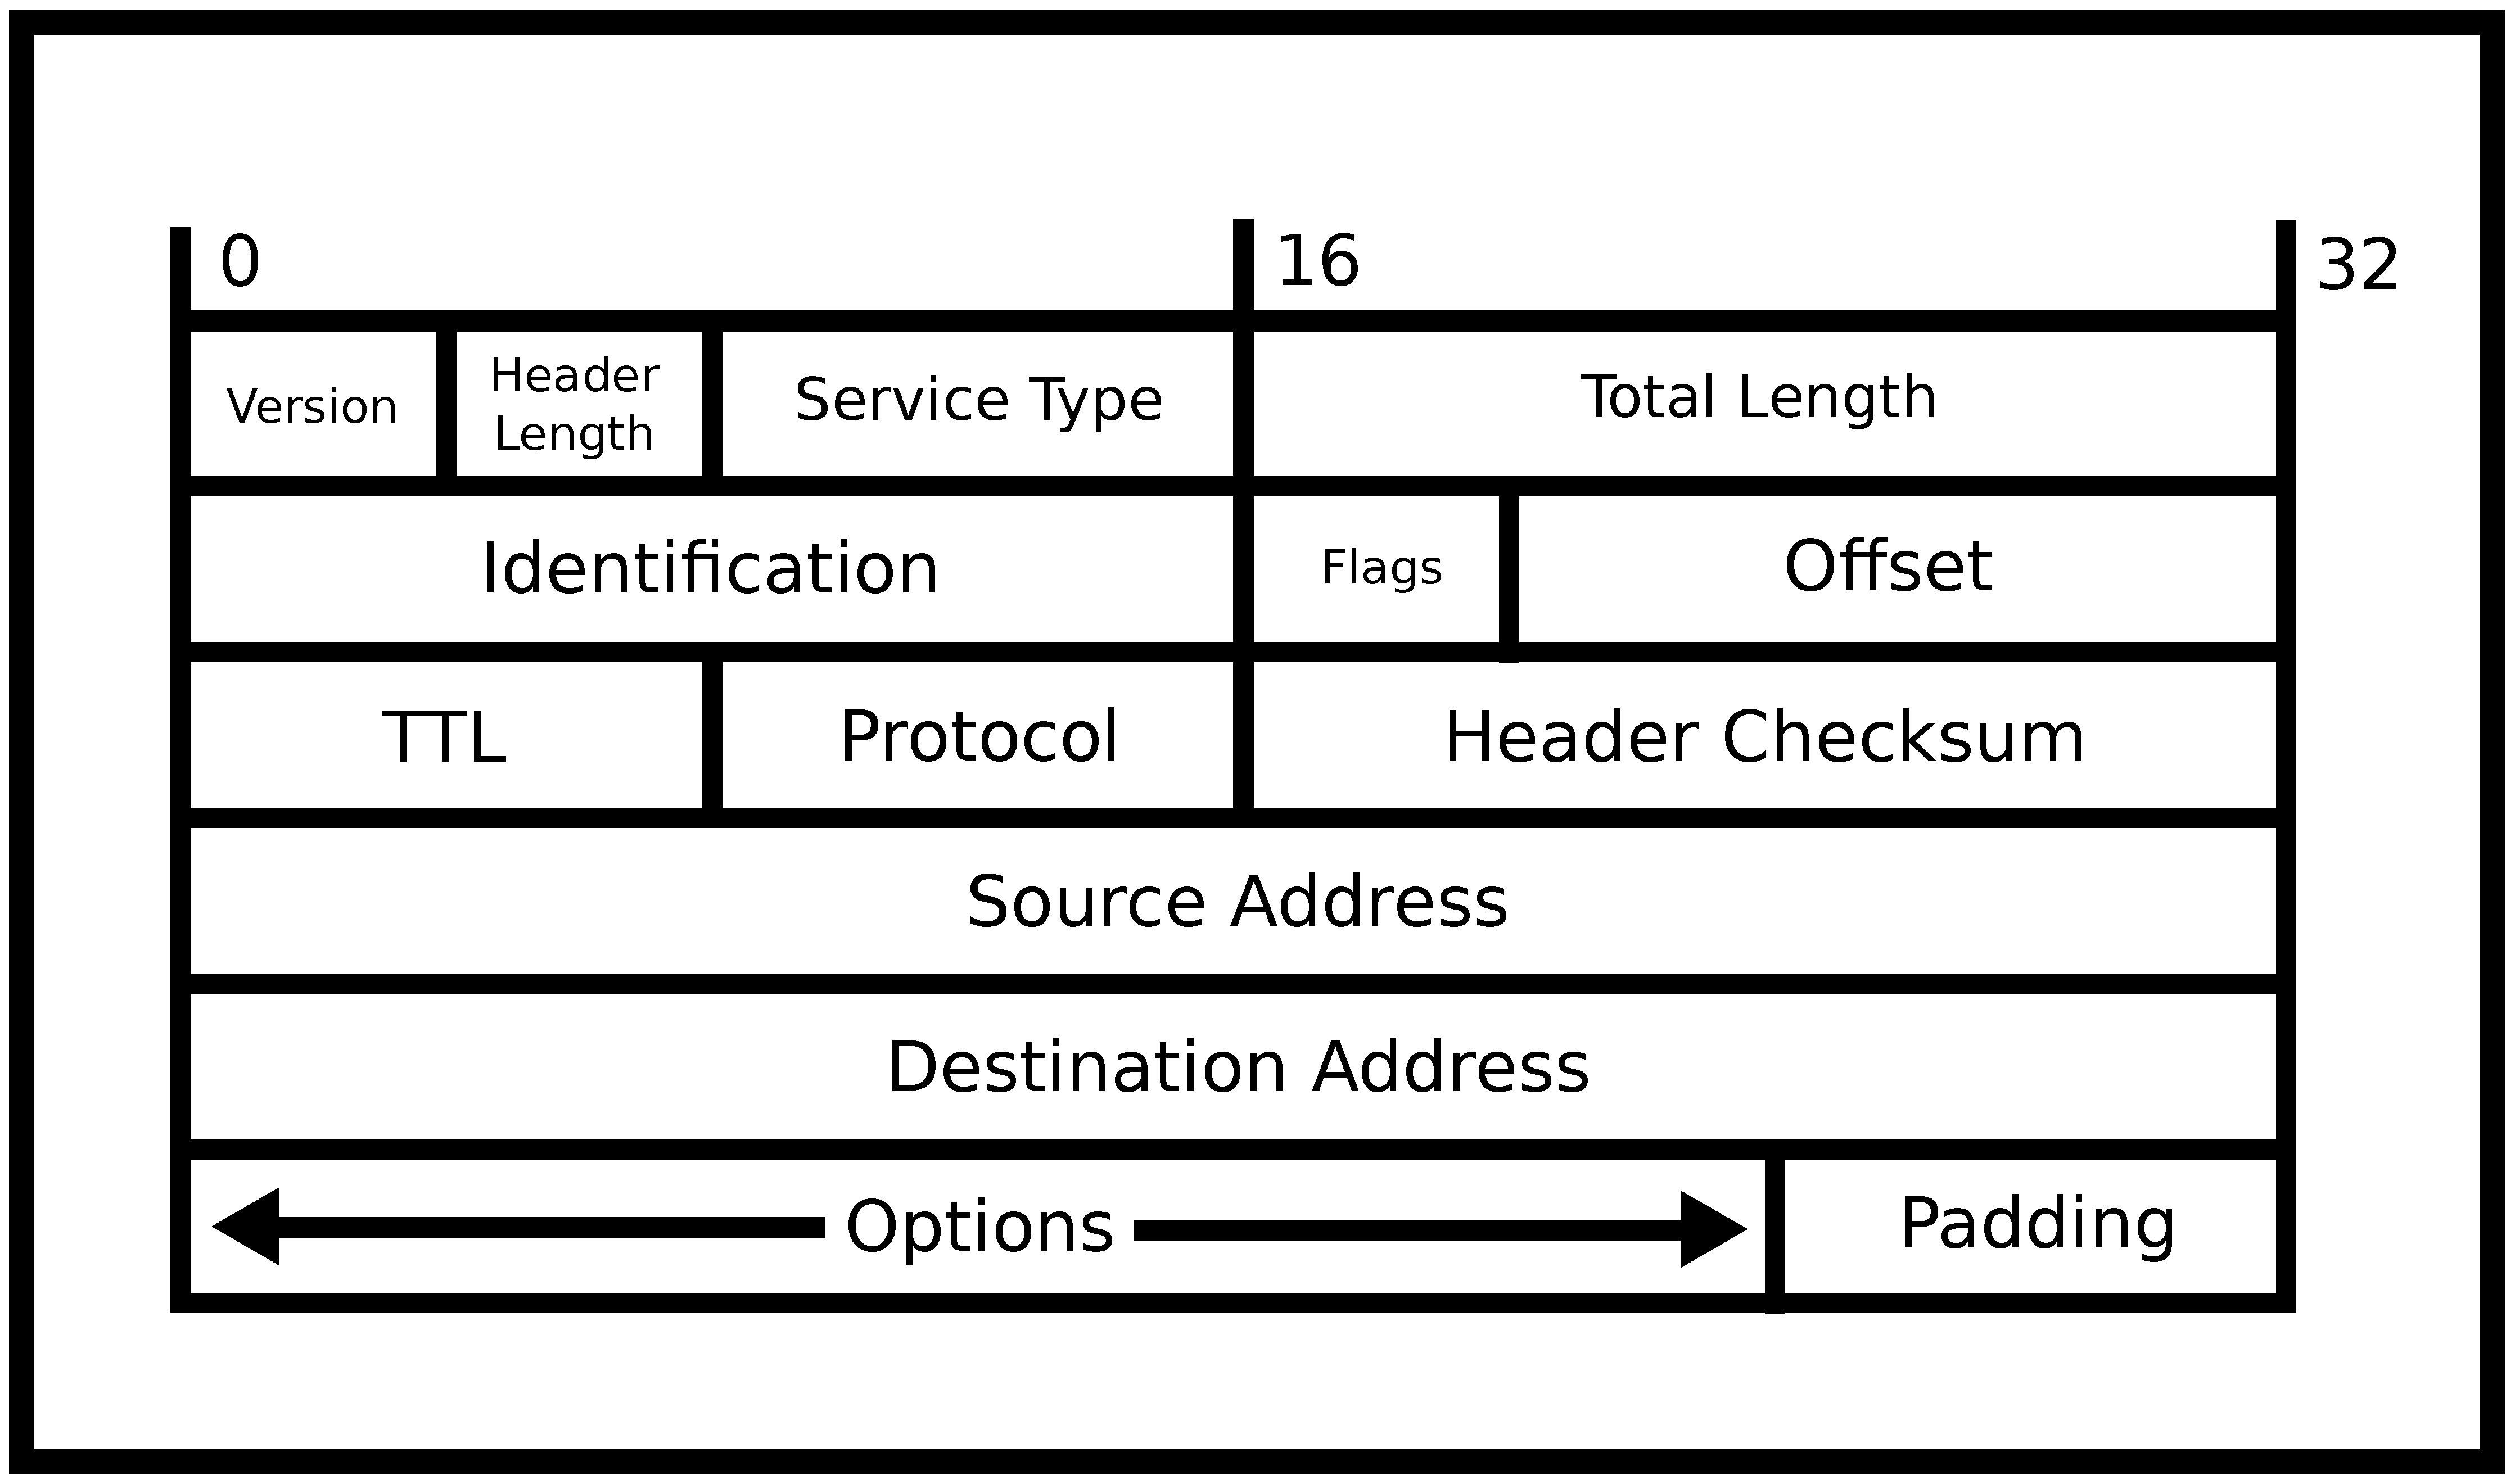
\includegraphics[width=.8\textwidth]{networking/drawings/ip_datagram.eps}
\caption{IP Datagram divisibility}
\end{figure}

\begin{enumerate}
  \item The first octet is the version number, either 4 or 6
  \item The next octet is how long the header is.
    Although it may seem that the header is constant size, you can include optional parameters to augment the path taken or other instructions
  \item The next two octets specify the total length of the datagram.
    This means this is the header, the data, footer, and padding.
    This is given in multiple of octets, meaning that a value of 20 means 20 octets.
  \item The next two are Identification number.
    IP handles taking packets that are too big to be sent over the physical wire and chunks them up.
    As such, this number identifies what datagram this originally belonged to.
  \item The next octet is various bit flags that can be set.
  \item The next octet and half is fragment number.
    If this packet was fragmented, this is the number this fragment represents
  \item The next octet is time to live.
    So this is the number of "hops" (travels over a wire) a packet is allowed to go.
    This is set because different routing protocols could cause packets to go in circles, the packets must be dropped at some point.
  \item The next octet is the protocol number.
    Although protocols between different layers of the OCI model are supposed to be black boxes, this is included, so that hardware can peer into the underlying protocol efficiently.
    Take for example IP over IP (yes you can do that!).
    Your ISP wraps IPv4 packets sent from your computer to the ISP in another IP layer and sends the packet off to be delivered to the website.
    On the reverse trip the packet is "unwrapped" and the original IP datagram is sent to your computer.
    This was done because we ran out of IP addresses, and this adds additional overhead but it is a necessary fix.
    Other common protocols are TCP, UDP, etc.
  \item The next two octets is an internet checksum.
    This is a CRC that is calculated to make sure that a wide variety of bit errors are detected.
  \item Source address is what people generally refer to as the IP address.
    There is no verification of this, so one host can pretend to be any IP address possible
  \item Destination address is where you want the packet to be sent to.
    This is crucial in the routing process as you need that to route.
  \item Additional options: Hosts of additional options, this is variadic in size.
  \item Footer: A bit of padding to make sure your data is a multiple of 4 octets.
  \item After: Your data! All data of higher order protocols are put following the header.
\end{enumerate}

\subsection{Extra: Routing}

The Internet Protocol routing is an amazing intersection of theory and application.
We can imagine the entire Internet as a set of graphs.
Most peers are connected to what we call "peering points" these are the WiFi routers and Ethernet ports that one finds in their house, work, or public.
These peering points are then connected to a wired network of routers, switches, and servers that all route themselves.
At a top level there are two types of routing

\begin{enumerate}
\item Internal Routing Protocols.
  Internal protocols is routing designed for within an ISP's network.
  These protocols are meant to be fast and more trusting because all computers, switches, and routers are part of an ISP.
  communication between two routers.
\item External Routing Protocols.
  These typically happen to be ISP to ISP protocol.
  Certain routers are designated as border routers.
  These routers talk to routers from ISPs have different policies from accepting or receiving packets.
  If an evil ISP is trying to dump all network traffic onto your ISP, these routers would deal with that.
  These protocols also deal with gathering information about the outside world to each router.
  In most routing protocols using link state or OSPF, a router must necessarily calculate the shortest path to the destination.
  This means it needs information about the "foreign" routers which is disseminated according to these protocols.
\end{enumerate}

These two protocols have to interplay with each other nicely in order to make sure that packets are mostly delivered.
In addition, ISPs need to be nice to each other because theoretically an ISP can handle lower load by forwarding all packets to another ISP.
If everyone does that then, no packets get delivered at all which won't make customers happy at all.
So these two protocols need to be fair so the end result works

If you want to read more about this, look at the Wikipedia page for routing here \href{https://en.wikipedia.org/wiki/Routing}{Routing}.

\subsection{Extra: Fragmentation/Reassembly}

Lower layers like WiFi and Ethernet have maximum transmission sizes.
The reason being is

\begin{enumerate}
  \item One host shouldn't crowd the medium for too long
  \item If an error occurs, we want some sort of "progress bar" on how far the communication has gone instead of retransmitting the entire stream.
  \item There are physical limitations, keeping a laser beam in optics working continuously may cause bit errors.
\end{enumerate}

If the Internet Protocol receives a packet that is too big for the maximum size, it must chunk it up.
TCP calculates how many datagrams that it needs to construct a packet and ensures that they are all transmitted and reconstructed at the end receiver.
The reason that we barely use this feature is that if any fragment is lost, the entire packet is lost.
Meaning that, assuming the probability of receiving a packet assuming each fragment is lost with an independent percentage, the probability of successfully sending a packet drops off exponentially as packet size increases.

As such, TCP slices its packets so that it fits inside on IP datagram.
The only time that this applies is when sending UDP packets that are too big, but most people who are using UDP optimize and set the same packet size as well.

\subsection{Extra: IP Multicast}

A little known feature is that using the IP protocol one can send a datagram to all devices connected to a router in what is called a multicast.
Multicasts can also be configured with groups, so one can efficiently slice up all connected routers and send a piece of information to all of them efficiently.
To access this in a higher protocol, you need to use UDP and specify a few more options.
Note that this will cause undue stress on the network, so a series of multicasts could flood the network fast.

\subsection{What's the deal with IPv6?}

\begin{figure}[H]
  \centering
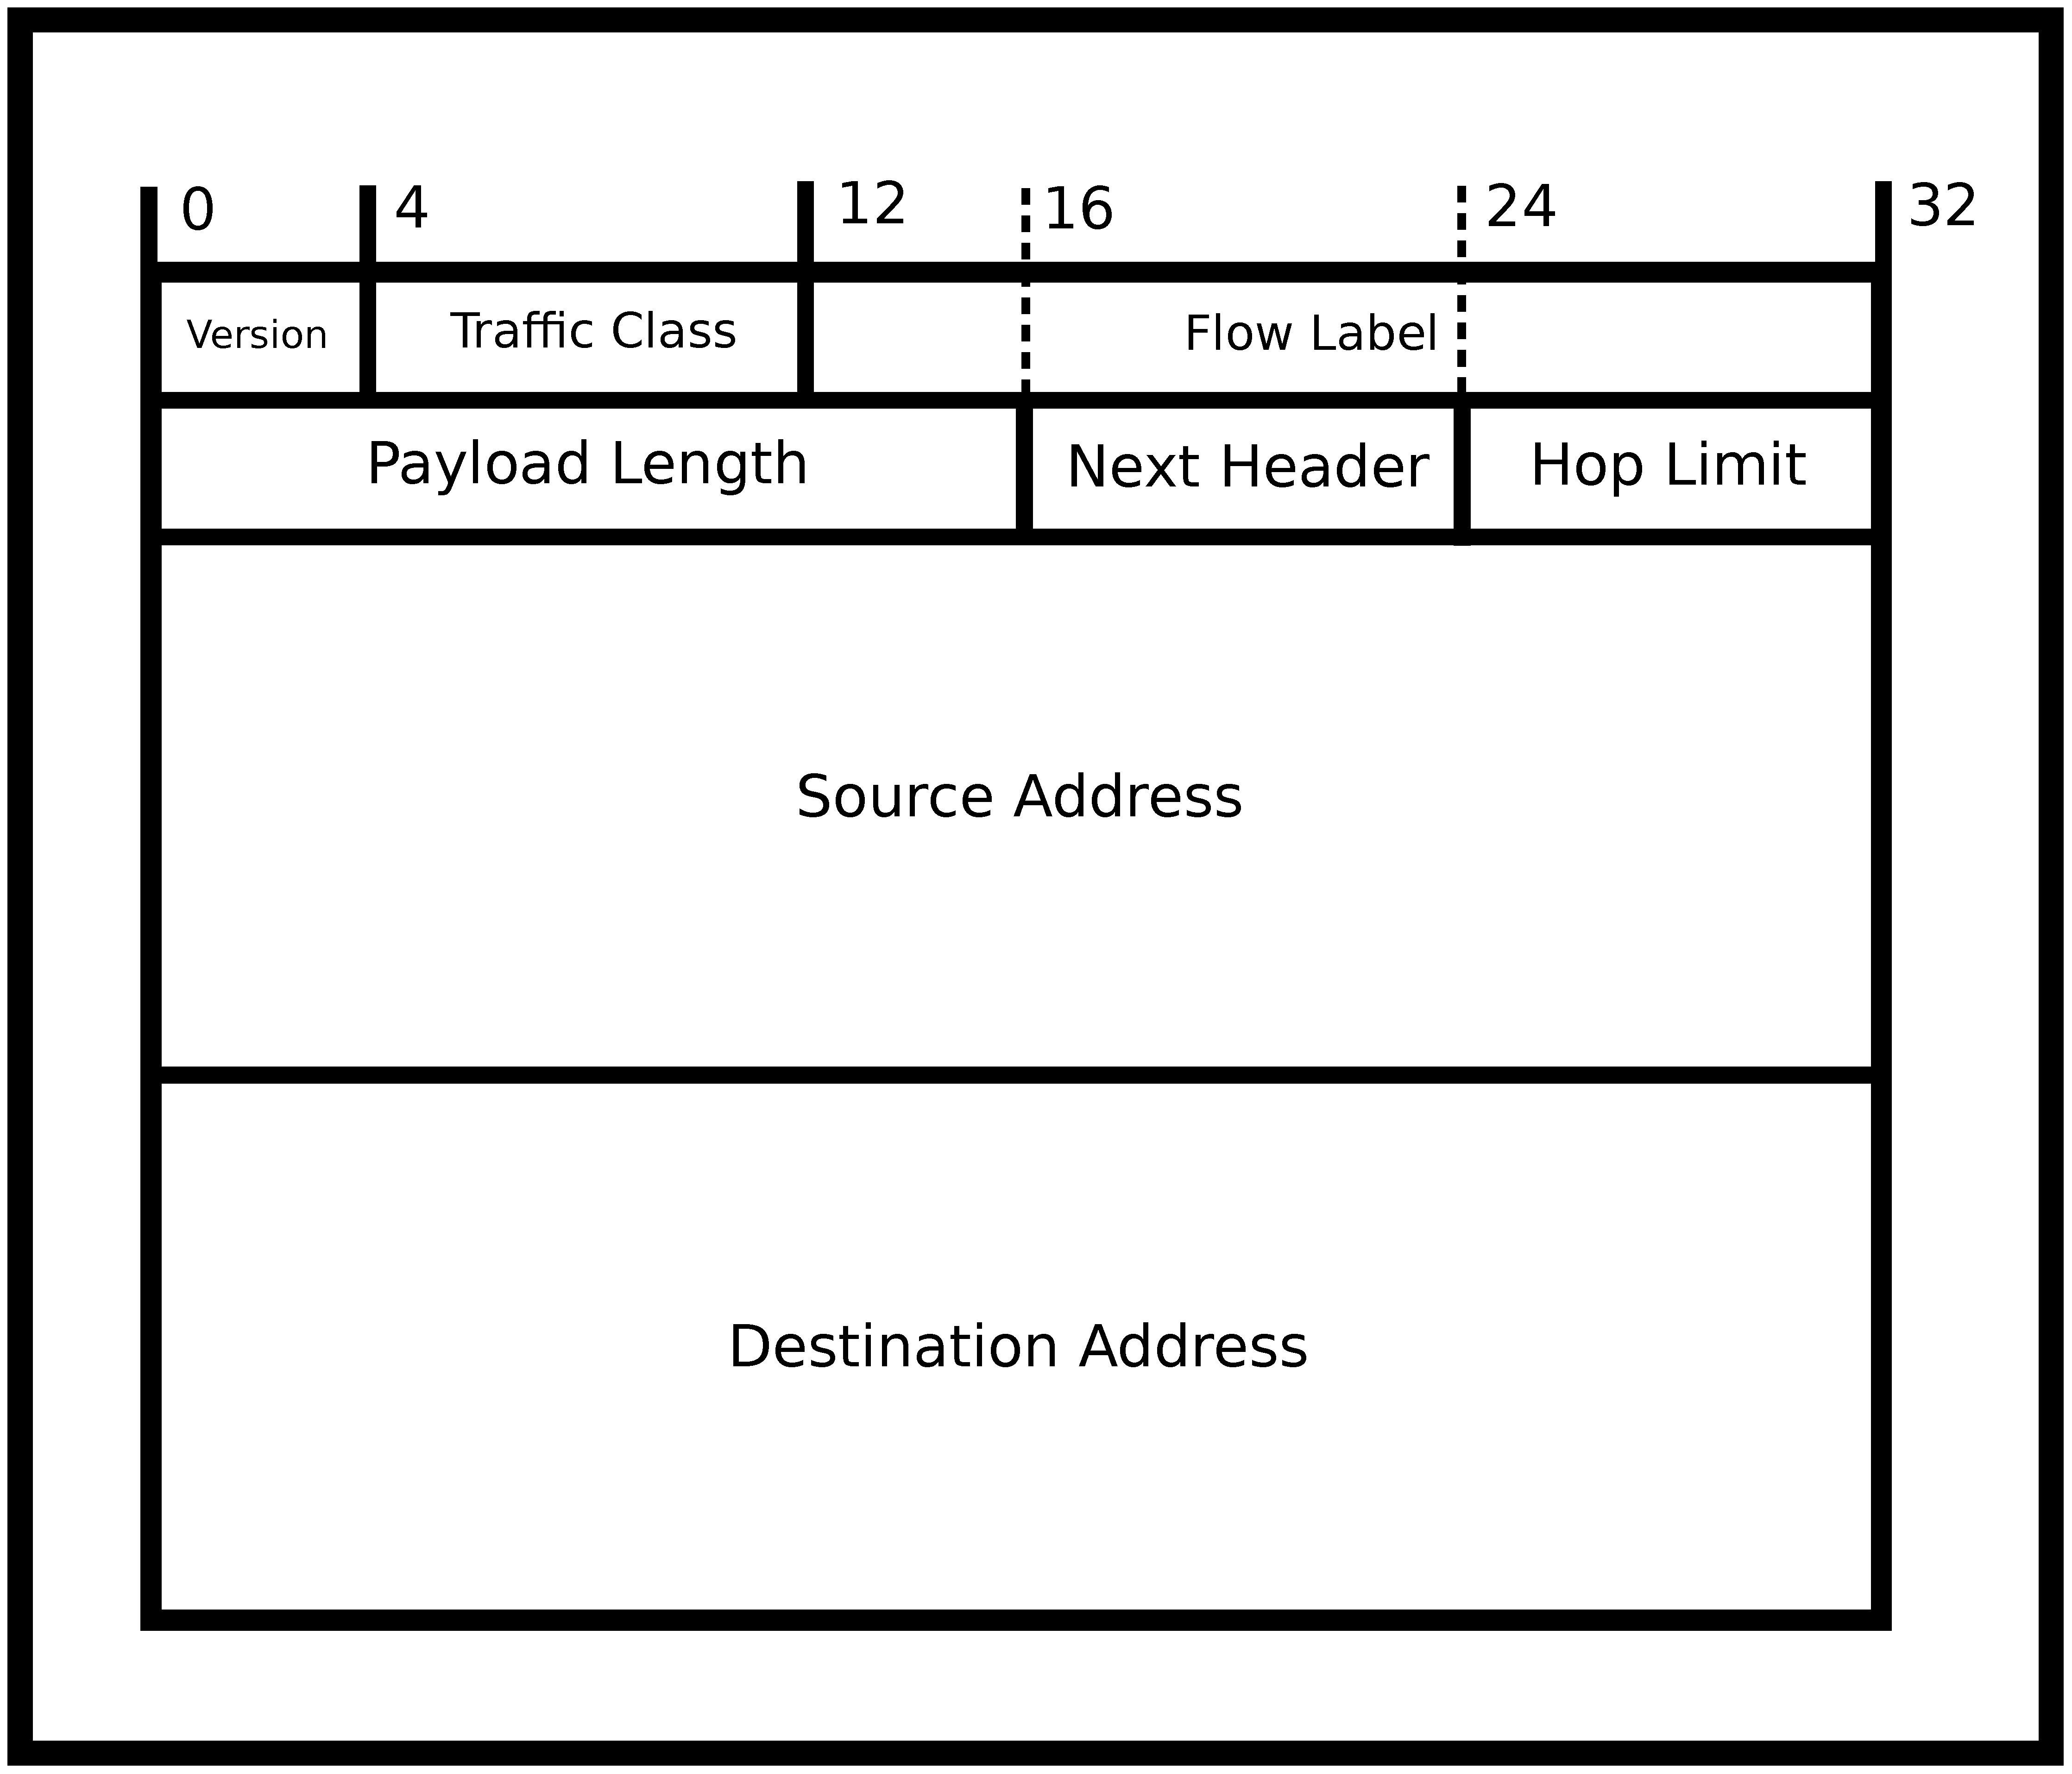
\includegraphics[width=.8\textwidth]{networking/drawings/ipv6_datagram.eps}
\caption{IPv6 Datagram divisibility}
\end{figure}

One of the big features of IPv6 is the address space.
The world ran out of IP addresses a while ago and has been using hacks to get around that.
With IPv6 there are enough internal and external addresses, so that unless we discover alien civilizations, we probably won't run out.
The other benefit is that these addresses are leased not bought, meaning that if something drastic happens in let's say the Internet of things and there needs to be a change in the block addressing scheme, it can be done.

Another big feature is security through IPsec.
IPv4 was designed with little to no security in mind.
As such, now there is a key exchange similar to TLS in higher layers that allows you to encrypt communication.

Another feature is simplified processing.
In order to make the Internet fast, IPv4 and IPv6 headers verification are actually implemented in hardware.
That means that all header options are processed in circuits as they come in.
The problem is that as the IPv4 spec grew to include a copious amount of headers, the hardware had to become more and more advanced to support those headers.
IPv6 reorders the headers so that packets can be dropped and routed with less hardware cycles.
In the case of the Internet, every cycle matters when trying to route the world's traffic.

\subsection{What's My Address?}

To obtain a linked list of IP addresses of the current machine use \keyword{getifaddrs} which will return a linked list of IPv4 and IPv6 IP addresses among other interfaces as well.
We can examine each entry and use \keyword{getnameinfo} to print the host's IP address.
The \keyword{ifaddrs} struct includes the family but does not include the sizeof the struct.
Therefore we need to manually determine the struct sized based on the family.

\begin{lstlisting}[language=C]
(family == AF_INET) ? sizeof(struct sockaddr_in) : sizeof(struct sockaddr_in6)
\end{lstlisting}

The complete code is shown below.

\begin{lstlisting}[language=C]
int required_family = AF_INET; // Change to AF_INET6 for IPv6
struct ifaddrs *myaddrs, *ifa;
getifaddrs(&myaddrs);
char host[256], port[256];

for (ifa = myaddrs; ifa != NULL; ifa = ifa->ifa_next) {
  int family = ifa->ifa_addr->sa_family;
  if (family == required_family && ifa->ifa_addr) {
    int ret = getnameinfo(ifa->ifa_addr,
    (family == AF_INET) ? sizeof(struct sockaddr_in) :
    sizeof(struct sockaddr_in6),
    host, sizeof(host), port, sizeof(port)
    , NI_NUMERICHOST | NI_NUMERICSERV)
    if (0 == ret) {
      puts(host);
    }
  }
}
\end{lstlisting}

To get your IP Address from the command line use \keyword{ifconfig} or Windows' \keyword{ipconfig}.

However, this command generates a lot of output for each interface, so we can filter the output using grep.

\begin{lstlisting}
ifconfig | grep inet

Example output:
    inet6 fe80::1%lo0 prefixlen 64 scopeid 0x1
    inet 127.0.0.1 netmask 0xff000000
    inet6 ::1 prefixlen 128
    inet6 fe80::7256:81ff:fe9a:9141%en1 prefixlen 64 scopeid 0x5
    inet 192.168.1.100 netmask 0xffffff00 broadcast 192.168.1.255
\end{lstlisting}

To actually grab the IP Address of a remote website, The function \keyword{getaddrinfo} can convert a human readable domain name (e.g. \keyword{www.illinois.edu}) into an IPv4 and IPv6 address.
In fact it will return a linked-list of addrinfo structs:

\begin{lstlisting}[language=C]
struct addrinfo {
  int              ai_flags;
  int              ai_family;
  int              ai_socktype;
  int              ai_protocol;
  socklen_t        ai_addrlen;
  struct sockaddr *ai_addr;
  char            *ai_canonname;
  struct addrinfo *ai_next;
};
\end{lstlisting}

For example, suppose you wanted to find out the numeric IPv4 address of a web server at \keyword{www.bbc.com}.
We do this in two stages.
First use getaddrinfo to build a linked-list of possible connections.
Secondly use \keyword{getnameinfo} to convert the binary address of one of those into a readable form.

\begin{lstlisting}[language=C]
#include <stdio.h>
#include <stdlib.h>
#include <sys/types.h>
#include <sys/socket.h>
#include <netdb.h>

struct addrinfo hints, *infoptr; // So no need to use memset global variables

int main() {
  hints.ai_family = AF_INET; // AF_INET means IPv4 only addresses

  // Get the machine addresses
  int result = getaddrinfo("www.bbc.com", NULL, &hints, &infoptr);
  if (result) {
    fprintf(stderr, "getaddrinfo: %s\n", gai_strerror(result));
    exit(1);
  }

  struct addrinfo *p;
  char host[256];

  for(p = infoptr; p != NULL; p = p->ai_next) {
    // Get the name for all returned addresses
    getnameinfo(p->ai_addr, p->ai_addrlen, host, sizeof(host), NULL, 0, NI_NUMERICHOST);
    puts(host);
  }

  freeaddrinfo(infoptr);
  return 0;
}
\end{lstlisting}

Possible output.

\begin{lstlisting}
212.58.244.70
212.58.244.71
\end{lstlisting}

In addition to specifying IPv4 or IPv6, one can specify either with \keyword{AF\_UNSPEC}.
Just replace the ai\_family attribute in the above code with the following.

\begin{lstlisting}
hints.ai_family = AF_UNSPEC
\end{lstlisting}

If you are wondering how the computer maps \gls{hostnames} to addresses, we will talk about that in Layer 7.
Spoiler: It is a service called \gls{DNS}.
Before we move onto the next section, it is important to note that a single website can have multiple IP addresses.
This may be to be efficient with machines.
If Google or Facebook has a single server routing \textit{all} of their incoming requests to other computers, they'd have to spend massive amounts of money on that computer or data center.
Instead they can give different regions different IP addresses and have a computer pick.
It isn't bad to access a website through the non-preferred IP address.
You may just get slower loading times.

\section{Layer 4: TCP and Client}


\begin{figure}[H]
  \centering
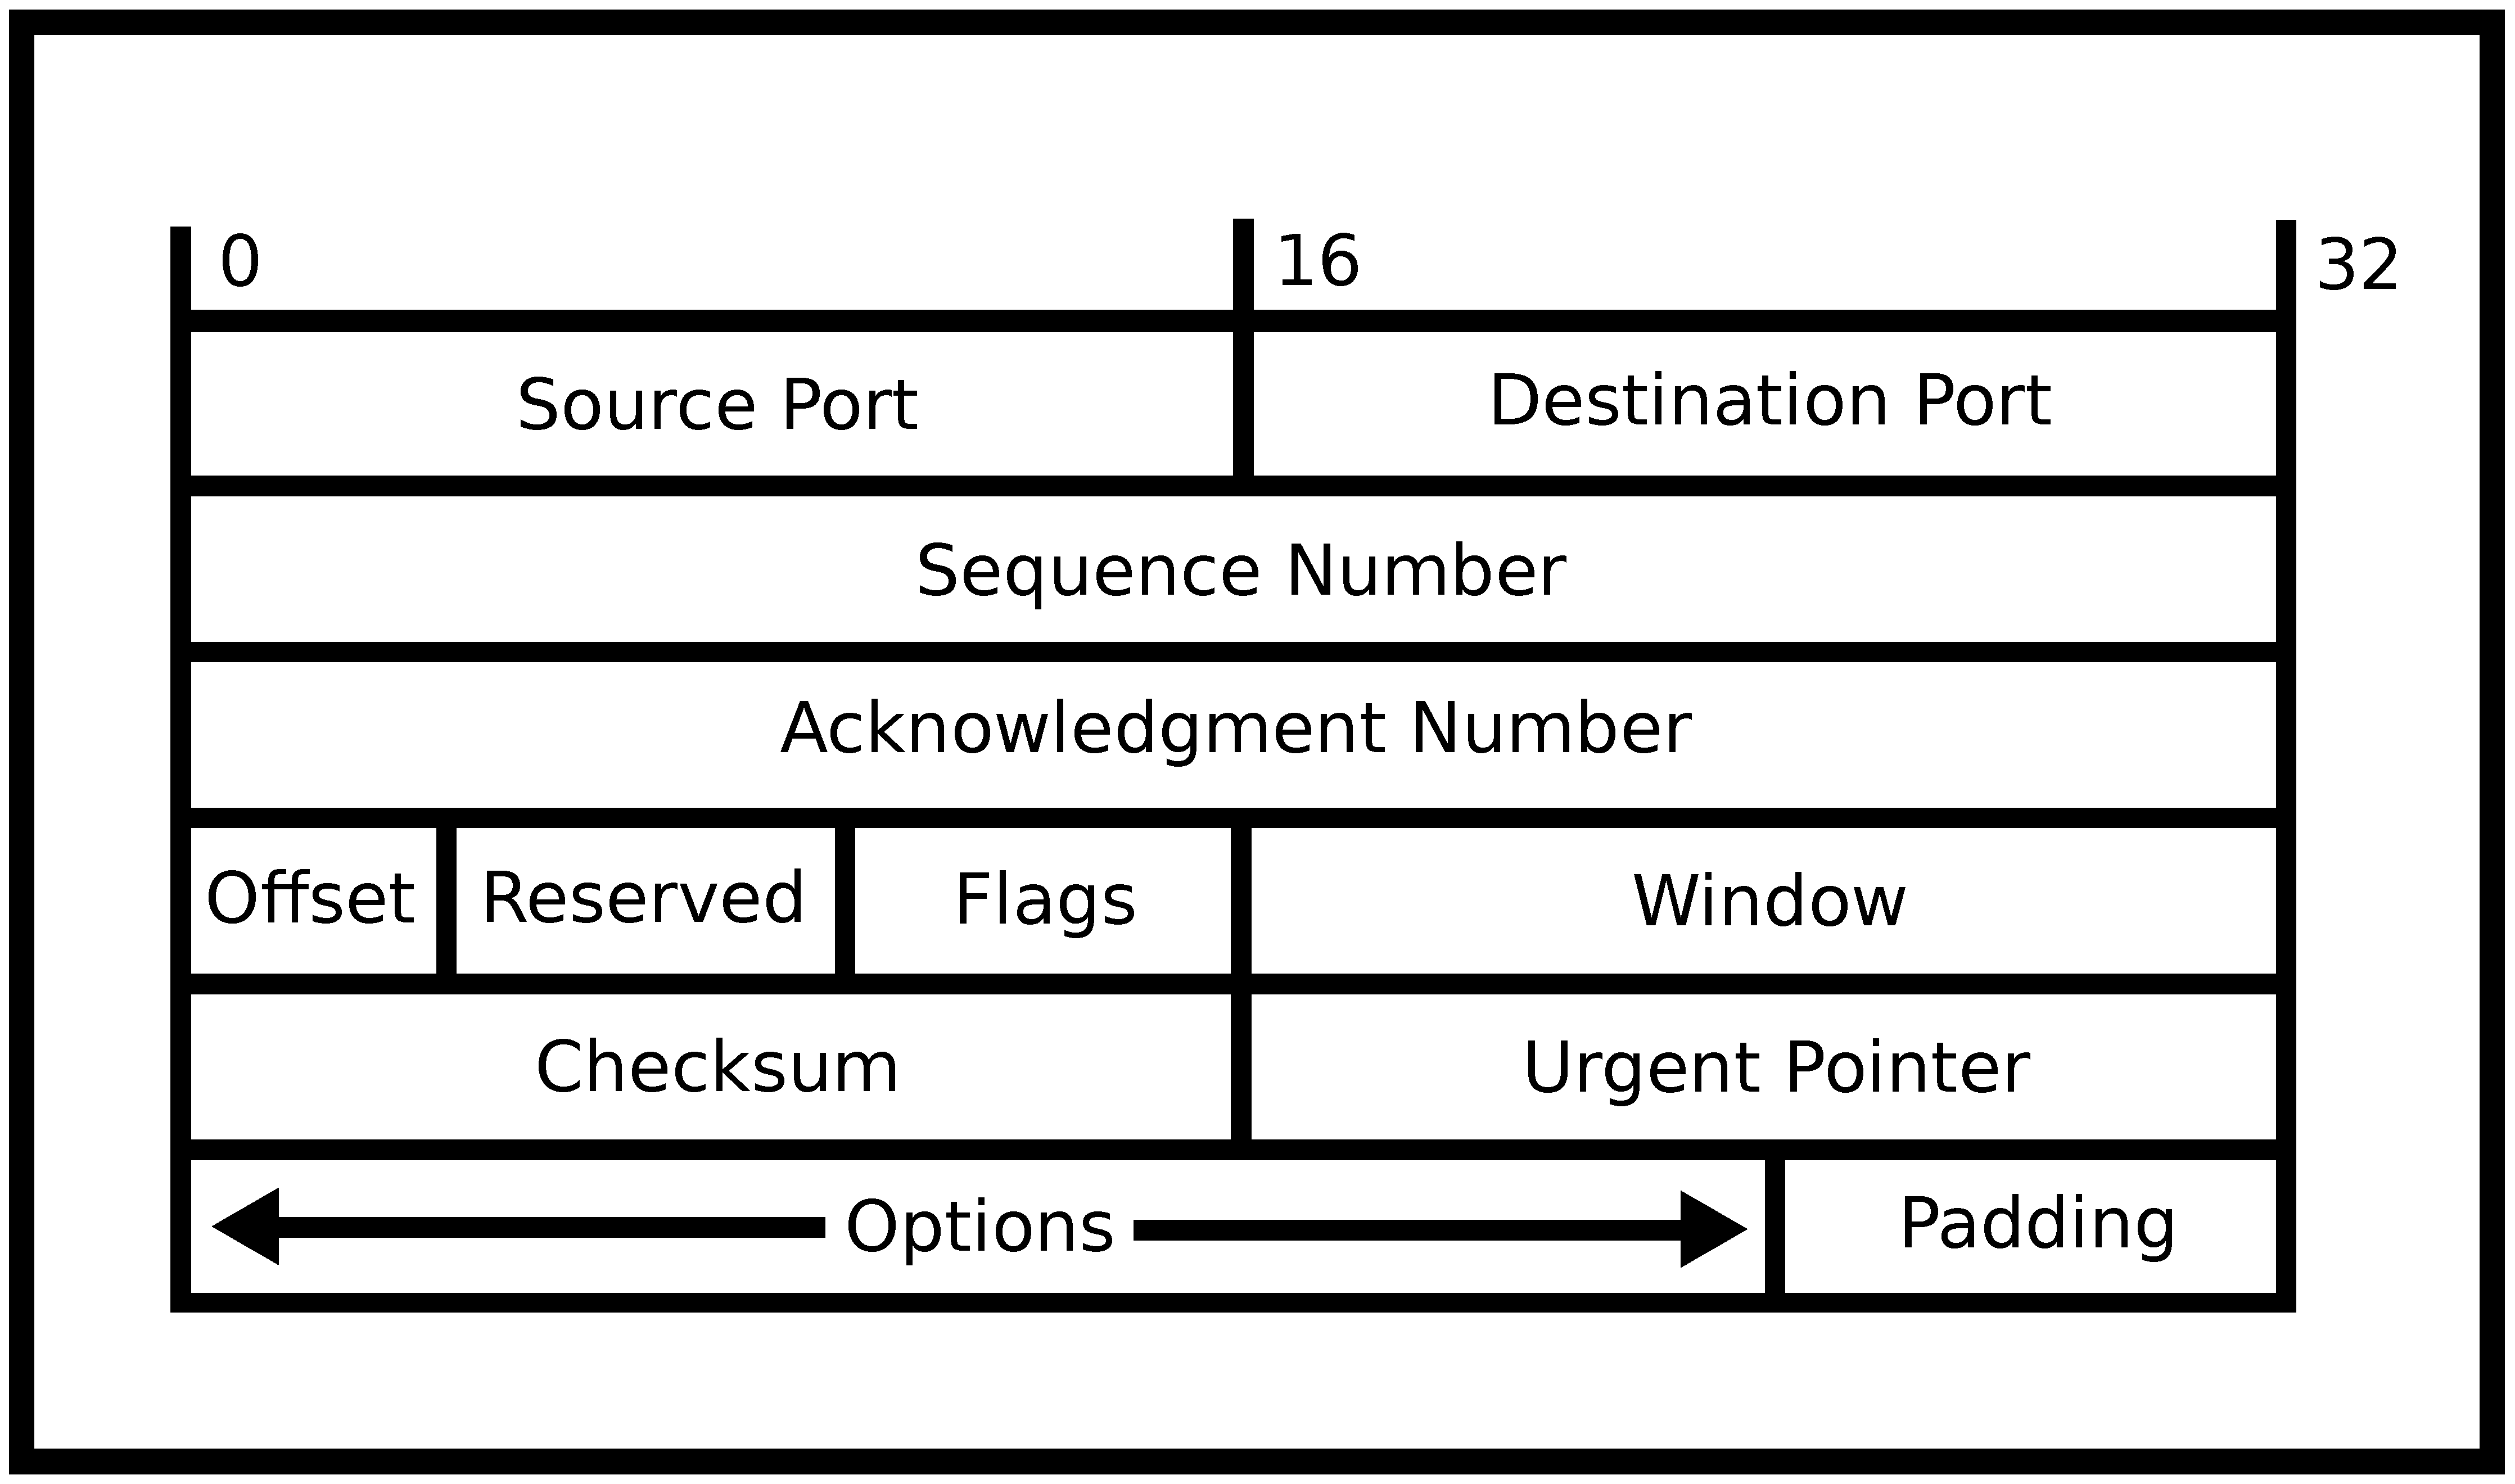
\includegraphics[width=.8\textwidth]{networking/drawings/tcp_header.eps}
\caption{Extra: TCP Header Specification}
\end{figure}

Most services on the Internet today use \gls{TCP} because it efficiently hides the complexity of lower, packet-level nature of the Internet.
TCP or Transport Control Protocol is a connection-based protocol that is built on top of IPv4 and IPv6 and therefore can be described as ``TCP/IP'' or ``TCP over IP''.
TCP creates a \emph{pipe} between two machines and abstracts away the low level packet-nature of the Internet. Thus, under most conditions, bytes sent over a TCP connection will not be lost or corrupted.

TCP has a number of features that set it apart from the other transport protocol UDP.

\begin{enumerate}
  \item \gls{Ports}
  With IP, you are only allowed to send packets to a machine.
  If you want one machine to handle multiple flows of data, you have to do it manually with IP.
  TCP abstracts that gives the programmer a set of virtual sockets.
  Clients specify the socket that you want the packet sent to and the TCP protocol makes sure that applications that are waiting for packets on that port receive that.
  A process can listen for incoming packets on a particular port.
  However, only processes with \gls{super-user} (root) access can listen on ports less than 1024.
  Any process can listen on ports 1024 or higher.
  An often used port is port 80: Port 80 is used for unencrypted HTTP requests or web pages.
  For example, if a web browser connects to \keyword{http://www.bbc.com/} then it will be connecting to port 80.

\item \gls{Retransmission}
  Packets can get dropped due to network errors or congestion.
  As such, they need to be retransmitted but at the same time the retransmission shouldn't cause packets more packets to be dropped.
  This needs to balance the tradeoff between flooding the network and speed.

\item Out of order packets.
  Packets may get routed more favorably due to various reasons in IP.
  If a later packet arrives before another packet, the protocol should detect and reorder them.

\item Duplicate packets.
  Packets can arrive twice.
  Packets can arrive twice.
  As such, a protocol need to be able to differentiate between two packets given a sequence number subject to overflow.

\item Error correction.
  There is a TCP checksum that handles bit errors.
  This is rarely used though.

\item Flow Control.
  Flow control is performed on the receiver side.
  This may be done so that a slow receiver doesn't get overwhelmed with packets.
  Servers especially that may handle 10000 or 10 million concurrent connections may need to tell receivers to slow down, but not disconnect due to load.
  There are also other problem of making sure the local network is not overwhelmed

\item Congestion control.
  Congestion control is performed on the sender side.
  Congestion control is to avoid a sender from flooding the network with too many packets.
  This is really important to make sure that each TCP connection is treated fairly.
  Meaning that two connections leaving a computer to google and youtube receive the same bandwidth and ping as each other.
  One can easily define a protocol that takes all the bandwidth and leaves other protocols in the dust, but this tends to be malicious because more often than not limiting a computer to a single TCP connection will yield the same result.

\item Connection oriented/life cycle oriented.
  You can really imagine a TCP connection as a series of bytes sent through a pipe.
  There is a ``lifecycle'' to a TCP connection though. What this means is that a TCP connection has a series of states and certain packets received can or not received can move it to another state.
  TCP handles setting up the connection through SYN SYN-ACK ACK. This means the client will send a SYNchronization packet that tells TCP what starting sequence to start on. Then the receiver will send a SYN-ACK message acknowledging the synchronization number.
  Then the client will ACKnowledge that with one last packet.
  The connection is now open for both reading and writing on both ends
  TCP will send data and the receiver of the data will acknowledge that it received a packet.
  Then every so often if a packet is not sent, TCP will trade zero length packets to make sure the connection is still alive.
  At any point, the client and server can send a FIN packet meaning that the server will not transmit.
  This packet can be altered with bits that only close the read or write end of a particular connection. When all ends are closed then the connection is over.
\end{enumerate}

There are a list of things that TCP doesn't provide though

\begin{enumerate}
\item Security.
  This means that if you connect to an IP address that says that it is a certain website, TCP does not verify that this website is in fact that IP address.
  You could be sending packets to a malicious computer.
\item Encryption.
  Anybody can listen in on plain TCP.
  The packets in transport are in plain text meaning that important things like your passwords could easily be skimmed by servers and regularly are.
\item Session Reconnection.
  This is handled by a higher protocols, but if a TCP connection dies then a whole new one must be created and the transmission has to be started over again.
\item Delimiting Requests.
  TCP is naturally connection oriented.
  Applications that are communicating over TCP need to find a unique way of telling each other that this request or response is over.
  HTTP delimits the header through two carriage returns and uses either a length field or one keeps listening until the connection closes
\end{enumerate}

\subsection{Note on network orders}

Integers can be represented in least significant byte first or most-significant byte first.
Either approach is reasonable as long as the machine itself is internally consistent.
For network communications, we need to standardize on agreed format.

\keyword{htons(xyz)} returns the 16-bit unsigned integer `short' value xyz in network byte order.
\keyword{htonl(xyz)} returns the 32-bit unsigned integer `long' value xyz in network byte order.
Any longer integers need to have the computers specify the order.

These functions are read as `host to network'.
The inverse functions (\keyword{ntohs}, \keyword{ntohl}) convert network ordered byte values to host-ordered ordering.
So, is host-ordering little-endian or big-endian?
The answer is - it depends on your machine!
It depends on the actual architecture of the host running the code.
If the architecture happens to be the same as network ordering then the result of these functions is just the argument.
For x86 machines, the host and network ordering is different.

Unless agreed otherwise whenever you read or write the low level C network structures, for example port and address information, remember to use the above functions to ensure correct conversion to/from a machine format.
Otherwise the displayed or specified value may be incorrect.

This doesn't apply to protocols that negotiate the endianness before-hand.
If two computers are CPU bound by converting the messages between network orders -- this happens with RPCs in high performance systems -- it may be worth it to negotiate if they are on similar endians to send in little endian order.

Why is network order defined to be big endian?
The simple answer is that RFC1700 says so \cite{RFC1700}.
If you want more information, we'll cite the famous article located that argued for a particular version \cite{cohen_1980}.
The most important part is that it is standard.
What happens when we don't have one standard?
We have 4 different USB plug types (Regular, Micro, Mini, and USB-C) that don't interact well with each other.
Obviously include relevant XKCD here.

\subsection{TCP Client}

There are three basic system calls you need to connect to a remote machine.

\begin{enumerate}

\item \keyword{int getaddrinfo(const char *node, const char *service,
                       const struct addrinfo *hints,
                       struct addrinfo **res);}

The \keyword{getaddrinfo} call if successful, creates a linked-list of \keyword{addrinfo} structs and sets the given pointer to point to the first one.

In addition, you can use the hints struct to only grab certain entries like certain IP protocols etc.
The addrinfo structure that is passed into \keyword{getaddrinfo} to define the kind of connection you'd like.
For example, to specify stream-based protocols over IPv6, you can use the following snippet.

\begin{lstlisting}[language=C]
struct addrinfo hints;
memset(&hints, 0, sizeof(hints));

hints.ai_family = AF_INET6; // Only want IPv6 (use AF_INET for IPv4)
hints.ai_socktype = SOCK_STREAM; // Only want stream-based connection
\end{lstlisting}

The other modes for family are \keyword{AF\_INET4} and \keyword{AF\_UNSPEC} which mean IPv4 and unspecified respectively.
This could be useful if you are searching for a service that you aren't entirely sure which IP version.
Naturally, you get the version in the field back if you specified UNSPEC.

Error handling with \keyword{getaddrinfo} is a little different.
The return value \emph{is} the error code.
To convert to a human-readable error use \keyword{gai\_strerror} to get the equivalent short English error text.

\begin{lstlisting}[language=C]
int result = getaddrinfo(...);
if(result) {
  const char *mesg = gai_strerror(result);
  ...
}
\end{lstlisting}


\item \keyword{int socket(int domain, int socket\_type, int protocol);}

The socket call creates a network socket and returns a descriptor that can be used with \keyword{read} and \keyword{write}.
In this sense it is the network analog of \keyword{open} that opens a file stream -- except that we haven't connected the socket to anything yet!

Sockets are created with a domain \keyword{AF\_INET} for \keyword{IPv4} or \keyword{AF\_INET6} for \keyword{IPv6}, \keyword{socket\_type} is whether to use UDP or TCP or other socket type, \keyword{protocol} is an optional choice of protocol configuration for our examples this we can just leave this as 0 for default.
This call creates a socket object in the kernel with which one can communicate with the outside world/network.
You can use the result of \keyword{getaddressinfo} to fill in the \keyword{socket} parameters, or provide them manually.

The socket call returns an integer - a file descriptor - and, for TCP clients, you can use it like a regular file descriptor.
You can use \keyword{read} and \keyword{write} to receive or send packets.

TCP sockets are similar to \keyword{pipes} and are often used in situations that require IPC.
We don't mention it in the previous chapters because it is overkill using a device suited for network to simply communicate between processes on a single thread.

\item \keyword{connect(int sockfd, const struct sockaddr *addr, socklen\_t addrlen);}

Finally the connect call attempts the connection to the remote machine.
We pass the original socket descriptor and also the socket address information which is stored inside the addrinfo structure.
There are different kinds of socket address structures which can require more memory.
So in addition to passing the pointer, the size of the structure is also passed.
To help identify errors and mistakes it is good practice to check the return value of all networking calls, including \keyword{connect}


\begin{lstlisting}[language=C]
// Pull out the socket address info from the addrinfo struct:
connect(sockfd, p->ai_addr, p->ai_addrlen)
\end{lstlisting}

\item (Optional) To clean up code call \keyword{freeaddrinfo(struct addrinfo *ai)} on the first level \keyword{addrinfo} struct.
\end{enumerate}

There is an old function \keyword{gethostbyname} is deprecated.
It's the old way convert a hostname into an IP address.
The port address still needs to be manually set using \keyword{htons} function.
It's much easier to write code to support IPv4 AND IPv6 using the newer \keyword{getaddrinfo}

This is all that is needed to create a \textit{simple} TCP client. However, network communications offers many different levels of abstraction and several attributes and options that can be set at each level of abstraction.
For example, we haven't talked about \keyword{setsockopt} which can manipulate options for the socket.
You can also mess around with lower layer protocols as the kernel provides primitives that contribute to this.
Note that you need to be root to create a raw socket.
In addition, you need to have a lot of ``set up'' or starter code, be prepared to have your datagrams be dropped due to bad form as well.
For more information see this \href{http://www.beej.us/guide/bgnet/output/html/multipage/getaddrinfoman.html}{guide}.

\subsection{Sending some data}

Once we have a successful connection we can read or write like any old file descriptor.
Keep in mind if you are connected to a website, you want to conform to the HTTP protocol specification in order to get any sort of meaningful results back.
There are libraries to do this, usually you don't connect at the socket level.
The number of bytes read or written may be smaller than expected.
Thus it is important to check the return value of read and write.
A simple HTTP client that sends a request to compliant URL is below.
First, we'll start with the boring stuff and the parsing code.

\begin{lstlisting}[language=C]
#include <stdio.h>
#include <stdlib.h>
#include <unistd.h>
#include <string.h>
#include <sys/types.h>
#include <sys/socket.h>
#include <netdb.h>
#include <errno.h>
#include <sys/types.h>
#include <sys/stat.h>
#include <fcntl.h>
#ifndef _GNU_SOURCE
#define _GNU_SOURCE
#endif

typedef struct _host_info {
  char *hostname;
  char *port;
  char *resource;
} host_info;

host_info *get_info(char *uri) {

  const char *http = "http://";
  int http_len = strlen(http);
  int uri_len = strlen(uri);
  if (uri_len < http_len && !strncmp(uri, http, min(strlen(http), uri_len))) {
    fprintf(stderr, "The uri must start with \"%s\"", http);
    exit(1);
  } else {
    uri += http_len;
    uri_len -= http_len;
  }
  char *hostname = malloc(uri_len+1);
  char *port = malloc(6);
  char *ptr = hostname;
  while(*uri && *uri != '/' && *uri != ':') {
    *ptr++ = *uri++;
  }
  *ptr = '\0';

  if(*uri == ':') {
    ptr = port;
    uri++;
    while(*uri != '/') {
      *ptr++ = *uri++;
    }
    *ptr = '\0';
  } else {
    free(port);
    port = strdup("80");
  }
  char *resource = NULL;
  int len = strlen(uri);
  if (len == 0) {
    // Empty means get the index
    resource = strdup("/");
  } else {
    resource = strdup(uri);
  }

  host_info *info = malloc(sizeof(*info));
  info->hostname = hostname;
  info->port = port;
  info->resource = resource;
  return info;
}

void free_info(host_info *info) {
  free(info->hostname);
  free(info->port);
  free(info->resource);
  free(info);
}

int main(int argc, char *argv[]) {
  if(argc != 2) {
    fprintf(stderr, "Usage: %s http://hostname[:port]/path\n", *argv);
    return 1;
  }
  char *uri = argv[1];
  host_info *info = get_info(uri);
  do {
    host_info *temp = send_request(info);
    free_info(info);
    info = NULL;
    if (temp) {
      info = temp;
    }
  } while(info);

  return 0;
}
\end{lstlisting}

The actual code that sends the request is below.
The first thing that we have to do is connect to an address.
We'll write up a nice helper function that does the error checking for us.

\begin{lstlisting}[language=C]
static void connect_to_address(int sock_fd, host_info *info) {
  struct addrinfo current, *result;
  memset(&current, 0, sizeof(struct addrinfo));
  current.ai_family = AF_INET;
  current.ai_socktype = SOCK_STREAM;
  int s = getaddrinfo(info->hostname, info->port, &current, &result);
  if (s != 0) {
    fprintf(stderr, "getaddrinfo: %s\n", gai_strerror(s));
    exit(1);
  }
  if(connect(sock_fd, result->ai_addr, result->ai_addrlen) == -1){
    perror("connection error");
    exit(1);
  }
  freeaddrinfo(result);
}
\end{lstlisting}

The next piece of code actually sends the request. Here is what each header means.

\begin{enumerate}
  \item "GET \%s HTTP/1.0" This is the request verb interpolated with the path. This means perform the GET verb on the path using the HTTP/1.0 method.
  \item "Connection: close" Means that as soon as the request is over, please close the connection. This line won't be used for any other connections.
    This is a little redundant given that HTTP 1.0 doesn't allow you to send multiple requests, but it is better to be explicit given there are non-conformant technologies.
  \item "Accept: */*" This means that the client is willing to accept anything.
\end{enumerate}

A more robust piece of code would also check if write fails or if the call was interrupted.

\begin{lstlisting}[language=C]
static void send_get_request(FILE *sock_file, host_info *info) {
  char *buffer;
  asprintf(&buffer,
  "GET %s HTTP/1.0\r\n"
  "Connection: close\r\n"
  "Accept: */*\r\n\r\n",
  info->resource);
  int sock_fd = fileno(sock_file);
  write(sock_fd, buffer, strlen(buffer));
  free(buffer);
}
\end{lstlisting}

The last piece of code is driver code that sends the request.
Feel free to use the following code if you want to open the file descriptor as a FILE object for convenience functions.
Just be careful not to forget to set the buffering to zero otherwise you may double buffer the input, which would lead to performance needs.

\begin{lstlisting}[language=C]
host_info *send_request(host_info *info) {
  int sock_fd = socket(AF_INET, SOCK_STREAM, 0);
  if (sock_fd == -1) {
    perror("socket");
    exit(1);
  }
  // Re-use address is a little overkill here because we are making a
  // Listen only server and we don't expect spoofed requests.
  int optval = 1;
  int retval = setsockopt(sock_fd, SOL_SOCKET, SO_REUSEADDR, &optval,
  sizeof(optval));
  if(retval == -1) {
    perror("setsockopt");
    exit(1);
  }
  connect_to_address(sock_fd, info);

  // Open so you can use getline
  FILE *sock_file = fdopen(sock_fd, "r+");
  setvbuf(sock_file, NULL, _IONBF, 0);

  send_get_request(sock_file, info);
  host_info *ret = NULL;
  if (is_redirect(sock_file)) {
    ret = handle_redirect(sock_file);
  } else {
    handle_okay(sock_file);
  }

  fclose(sock_file);
  return ret;
}
\end{lstlisting}

The example above demonstrates a request to the server using Hypertext Transfer Protocol.
In General, there are six parts

\begin{enumerate}
\item The method. GET,POST,\ldots{}
\item The resource. ``/'' ``/index.html'' ``/image.png''
\item The protocol ``HTTP/1.0''
\item A new line (\keyword{\\r\\n}). Requests always have a carriage return.
\item Any other knobs or switch parameters
\item The actual body of the request delimited by two new lines. The body of the request is either if the size is specified or until the receiver closes their connection.
\end{enumerate}

The server's first response line describes the HTTP version used and whether the request is successful using a 3 digit response code.

\begin{lstlisting}
HTTP/1.1 200 OK
\end{lstlisting}

If the client had requested a non existing file, e.g.
\keyword{GET /nosuchfile.html HTTP/1.0} Then the first line includes the response code is the well-known \keyword{404} response code.

\begin{lstlisting}
HTTP/1.1 404 Not Found
\end{lstlisting}

\todo{Cite RFC 7231 about message syntax and content}

\section{Layer 4: TCP Server}

The minimal four system calls required to create a TCP server are \keyword{socket}, \keyword{bind} \keyword{listen} and \keyword{accept}.
Each has a specific purpose and should be called in roughly the above order

\begin{enumerate}

  \item \keyword{int socket(int domain, int socket\_type, int protocol)}

  To create an endpoint for networking communication.
  A new socket by itself is not particularly useful.
  Though we've specified either a packet or stream-based connections, it is not bound to a particular network interface or port.
  Instead socket returns a network descriptor that can be used with later calls to bind, listen and accept.

  As one gotcha, these sockets must be declared passive.
  Passive server sockets do not actively try to connect to another host.
  Instead, they wait for incoming connections.
  Additionally, server sockets are not closed when the peer disconnects.
  Instead, the client communicates with a separate active socket on the server that is specific to that connection.

  Since a TCP connection is defined by the sender address and port along with a receiver address and port, a particular server port there can be one passive server socket but multiple active sockets.
  One for each currently open connection.
  The server's operating system maintains a lookup table that associates a unique tuple with active sockets, so that incoming packets can be correctly routed to the correct socket.

  \item \keyword{int bind(int sockfd, const struct sockaddr *addr, socklen\_t addrlen);}

  The \keyword{bind} call associates an abstract socket with an actual network interface and port.
  It is possible to call bind on a TCP client.
  The port information used by bind can be set manually (many older IPv4-only C code examples do this), or be created using \keyword{getaddrinfo}.

  By default a port is not immediately released when the server socket is closed.
  Instead, the port enters a ``TIMED-WAIT'' state.
  This can lead to significant confusion during development because the timeout can make valid networking code appear to fail.

  To be able to immediately reuse a port, specify \keyword{SO\_REUSEPORT} before binding to the port.

  \begin{lstlisting}[language=C]
  int optval = 1;
  setsockopt(sfd, SOL_SOCKET, SO_REUSEPORT, &optval, sizeof(optval));

  bind(...);
  \end{lstlisting}

  Here's \href{http://stackoverflow.com/questions/14388706/socket-options-so-reuseaddr-and-so-reuseport-how-do-they-differ-do-they-mean-t}{an extended stackoverflow introductory discussion of \keyword{SO\_REUSEPORT}}.

  \item \keyword{int listen(int sockfd, int backlog);}

    The \keyword{listen} call specifies the queue size for the number of incoming, unhandled connections.
    There are the connections that have not yet been assigned a network descriptor by \keyword{accept}.
    Typical values for a high performance server are 128 or more.

  \item \keyword{int accept(int sockfd, struct sockaddr *addr, socklen\_t *addrlen);}

  Once the server socket has been initialized the server calls \keyword{accept} to wait for new connections.
  Unlike \keyword{socket} \keyword{bind} and \keyword{listen}, this call will block, unless the non blocking option has been set.
  If there are no new connections, this call will block and only return when a new client connects.
  The returned TCP socket is associated with a particular tuple \keyword{(client IP, client port, server IP, server port)} and will be used for all future incoming and outgoing TCP packets that match this tuple.

  Note the \keyword{accept} call returns a new file descriptor.
  This file descriptor is specific to a particular client.
  It is a common programming mistake to use the original server socket descriptor for server I/O and then wonder why networking code has failed.

  The \keyword{accept} system call can optionally provide information about the remote client, by passing in a sockaddr struct.
  Different protocols have different variants of the \keyword{struct sockaddr}, which are different sizes.
  The simplest struct to use is the \keyword{sockaddr\_storage} which is sufficiently large to represent all possible types of sockaddr.
  Notice that C does not have any model of inheritance.
  Therefore we need to explicitly cast our struct to the `base type' struct sockaddr.

  \begin{lstlisting}[language=C]
  struct sockaddr_storage clientaddr;
  socklen_t clientaddrsize = sizeof(clientaddr);
  int client_id = accept(passive_socket,
  (struct sockaddr *) &clientaddr,
  &clientaddrsize);
  \end{lstlisting}

  We've already seen \keyword{getaddrinfo} that can build a linked list of addrinfo entries and each one of these can include socket configuration data.
  What if we wanted to turn socket data into IP and port addresses?
  Enter \keyword{getnameinfo} that can be used to convert a local or remote socket information into a domain name or numeric IP.
  Similarly, the port number can be represented as a service name.
  For example, port 80 is commonly used as the incoming connection port for incoming HTTP requests.
  In the example below, we request numeric versions for the client IP address and client port number.

  \begin{lstlisting}[language=C]
  socklen_t clientaddrsize = sizeof(clientaddr);
  int client_id = accept(sock_id, (struct sockaddr *) &clientaddr, &clientaddrsize);
  char host[NI_MAXHOST], port[NI_MAXSERV];
  getnameinfo((struct sockaddr *) &clientaddr,
  clientaddrsize, host, sizeof(host), port, sizeof(port),
  NI_NUMERICHOST | NI_NUMERICSERV);
  \end{lstlisting}

  One can use the macros \keyword{NI\_MAXHOST} to denote the maximum length of a hostname, and \keyword{NI\_MAXSERV} to denote the maximum length of a port.
  \keyword{NI\_NUMERICHOST} gets the hostname as a numeric IP address and similarly for \keyword{NI\_NUMERICSERV} though the port is usually numeric to begin with.
  The \href{https://man.openbsd.org/getnameinfo.3#NI\_NUMERICHOST}{Open BSD man pages have more information}

  \item \keyword{int close(int fd)} and \keyword{int shutdown(int fd, int how)}

  Use the \keyword{shutdown} call when you no longer need to read any more data from the socket, write more data, or have finished doing both.
  When you shutdown a socket for further writing or reading, that information is also sent to the other end of the connection.
  For example if you shutdown the socket for further writing at the server end, then a moment later, a blocked \keyword{read} call could return 0 to indicate that no more bytes are expected.
  Similarly a write to a a TCP connection that has been shutdown for reading will generate a SIGPIPE

  Use \keyword{close} when your process no longer needs the socket file descriptor.

  If you \keyword{fork}-ed after creating a socket file descriptor, all processes need to close the socket before the socket resources can be reused.
  If you shutdown a socket for further read, all process are be affected because you've changed the socket, not just the file descriptor.
  Well written code will \keyword{shutdown} a socket before calling \keyword{close} it.

\end{enumerate}

There are a few gotchas to creating a server.

\begin{itemize}
\item
  Using the socket descriptor of the passive server socket (described above)
\item
  Not specifying SOCK\_STREAM requirement for getaddrinfo
\item
  Not being able to reuse an existing port.
\item
  Not initializing the unused struct entries
\item
  The \keyword{bind} call will fail if the port is currently in use. Ports are per machine -- not per process or user.
  In other words, you cannot use port 1234 while another process is using that port.
  Worse, ports are by default `tied up' after a process has finished.
\end{itemize}

\subsection{Server code example}

A working simple server example is shown below.
Note this example is incomplete - for example it does not close either socket descriptor, or free up memory created by \keyword{getaddrinfo}

\begin{lstlisting}[language=C]
#include <string.h>
#include <stdio.h>
#include <stdlib.h>
#include <sys/types.h>
#include <sys/socket.h>
#include <netdb.h>
#include <unistd.h>
#include <arpa/inet.h>

int main(int argc, char **argv) {
  int s;

  // Create the socket!
  int sock_fd = socket(AF_INET, SOCK_STREAM, 0);

  // Grab the IP address
  struct addrinfo hints, *result;
  memset(&hints, 0, sizeof(struct addrinfo));
  hints.ai_family = AF_INET;
  hints.ai_socktype = SOCK_STREAM;
  hints.ai_flags = AI_PASSIVE;

  s = getaddrinfo(NULL, "1234", &hints, &result);
  if (s != 0) {
    fprintf(stderr, "getaddrinfo: %s\n", gai_strerror(s));
    exit(1);
  }

  // Bind and listen
  if (bind(sock_fd, result->ai_addr, result->ai_addrlen) != 0) {
    perror("bind()");
    exit(1);
  }

  if (listen(sock_fd, 10) != 0) {
    perror("listen()");
    exit(1);
  }

  struct sockaddr_in *result_addr = (struct sockaddr_in *) result->ai_addr;
  printf("Listening on file descriptor %d, port %d\n", sock_fd, ntohs(result_addr->sin_port));

  // Waiting for connections like a passive socket
  printf("Waiting for connection...\n");
  int client_fd = accept(sock_fd, NULL, NULL);
  printf("Connection made: client_fd=%d\n", client_fd);

  char buffer[1000];
  // Could get interrupted
  int len = read(client_fd, buffer, sizeof(buffer) - 1);
  buffer[len] = '\0';

  printf("Read %d chars\n", len);
  printf("===\n");
  printf("%s\n", buffer);

  return 0;
}
\end{lstlisting}

\subsection{Sorry to interrupt}

One concept that we need to make very clear is that you need to handle interrupts in your networking code.
That means that the sockets or accepted file descriptors that you read to or write to may have their calls interrupted -- most of the time you will get an interrupt or two.
In reality, any of your system calls could get interrupted.
The reason we bring this up now is that you are usually waiting for the network.
Which is an order of magnitude slower than processes.
Meaning a higher probability of getting interrupted.

How would you handle interrupts?
Let's try a quick example.

\begin{lstlisting}[language=C]
while bytes_read isn't count {
  bytes_read += read(fd, buf, count);
  if error is EINTR {
    continue;
  } else {
    break;
  }
}
\end{lstlisting}

We can assure you that the following code \textit{will not work}.
Can you see why?
At the surface level it does restart a call after a read or write.
But what else happens when the error is EINTR?
Is the contents of the buffer correct?
What other problems can you spot?

\section{Layer 4: UDP}

UDP is a connectionless protocol that is built on top of IPv4 and IPv6.
It's very simple to use.
Decide the destination address and port and send your data packet!
However, the network makes no guarantee about whether the packets will arrive.
Packets may be dropped if the network is congested.
Packets may be duplicated or arrive out of order.

A typical use case for UDP is when receiving up to date data is more important than receiving all of the data.
For example, a game may send continuous updates of player positions.
A streaming video signal may send picture updates using UDP

\subsection{UDP Attributes}

\begin{itemize}
\item Unreliable Datagram Protocol
  Packets sent through UDP are not guaranteed to reach their destination.
  The probability that the packet gets delivered goes down over time.
  This can especially be confusing because if you only test on your loop-back device -- this is localhost or 127.0.0.1 for most users -- then there will almost never be loss because no network packets are sent.
\item Simple
  The UDP protocol is supposed to have much less fluff than TCP.
  Meaning that for TCP there are a lot of configurable parameters and a lot of edge cases in the implementation.
  UDP is just fire and forget.
\item Stateless/Transaction
  The UDP protocol does not keep a ``state'' of the connection.
  This makes the protocol more simple and let's the protocol represent simple transactions like requesting or responding to queries.
  There is also less overhead to sending a UDP message because there is no three way handshake.
\item Manual Flow/Congestion Control
  You have to manually manage the flow and congestion control which is a double edged sword.
  On one hand you have full control over everything, but on the other hand TCP has \textit{decades} of optimization, meaning your protocol for its use cases needs to be more efficient that to be more beneficial to use it.
\item Multicast
  This is one thing that you can only do with UDP.
  This means that you can send a message to every peer connected to a particular router that is part of a particular group.
\end{itemize}

\todo{Include the main UDP RFC}

While it may seem that you never want to use UDP for situations that you don't want to lose data, a lot of protocols base their communication based on UDP that require no data loss.
Take a look at the Trivial File Transfer Protocol that reliably transmits a file over the wire using UDP only.
Of course there is more configuration involved, but choosing between UDP over TCP isn't just the above factors.

\subsection{UDP Client}

UDP Clients are pretty versatile below is a simple client that sends a packet to a server specified through the command line.
Note that this client sends a packet and doesn't wait for acknowledgement.
It fires and forgets.
The example below also uses \keyword{gethostbyname} because some legacy functionality still works pretty well for setting up a client.

\begin{lstlisting}[language=C]
struct sockaddr_in addr;
memset(&addr, 0, sizeof(addr));
addr.sin_family = AF_INET;
addr.sin_port = htons((uint16_t)port);
struct hostent *serv = gethostbyname(hostname);
if (!serv) {
  perror("gethostbyname");
  exit(1);
}
\end{lstlisting}

The previous code grabs an entry \keyword{hostent} that matches by hostname.
Even though this isn't portable, it definitely gets the job done.
The full example follows.

\begin{lstlisting}[language=C]
// Relevant headers ..

int connect_to_udp(int port, char *hostname, struct sockaddr_in *ipaddr) {
  int sockfd = socket(AF_INET, SOCK_DGRAM, 0);
  if (sockfd < 0) {
    perror("socket");
    exit(1);
  }
  int optval = 1;
  setsockopt(sockfd, SOL_SOCKET, SO_REUSEPORT, &optval, sizeof(optval));

  // Get host by name TODO: Refactor to getaddrinfo
  struct sockaddr_in addr;
  memset(&addr, 0, sizeof(addr));
  addr.sin_family = AF_INET;
  addr.sin_port = htons((uint16_t)port);
  struct hostent *serv = gethostbyname(hostname);
  if (!serv) {
    perror("gethostbyname");
    exit(1);
  }

  // Full definitions of the structs are provided in the man
  // pages so it is safe to copy them over
  // meaning they aren't meant to be opaque types
  memcpy(&addr.sin_addr.s_addr, serv->h_addr, serv->h_length);

  if (ipaddr) {
    memcpy(ipaddr, &addr, sizeof(*ipaddr));
  }

  // Timeouts for resending acks and whatnot
  struct timeval tv;
  tv.tv_sec = 0;
  tv.tv_usec = SOCKET_TIMEOUT;
  setsockopt(sockfd, SOL_SOCKET, SO_RCVTIMEO, &tv, sizeof(tv));

  return sockfd;
}

// later

int port_fd = connect_to_udp(port, hostname, &ipaddr, 0)
char *to_send = "Hello!"

// sendto may error, but that isn't because the packet wasn't
// delivered. There could be bad addresses, bad port sends etc
int send_ret = sendto(port_fd, to_send, packet_size, 0,
(struct sockaddr *)&ipaddr,
sizeof(ipaddr));
\end{lstlisting}

The above code simply sends ``Hello'' through a UDP. There is no idea of if the packet arrives, is processed etc.

\subsection{UDP Server}

There are a variety of function calls available to send UDP sockets.
We will use the newer \keyword{getaddrinfo} to help set up a socket structure.
Remember that UDP is a simple packet-based (`datagram') protocol. There is no connection to set up between the two hosts.
First, initialize the hints addrinfo struct to request an IPv6, passive datagram socket.

\begin{lstlisting}[language=C]
memset(&hints, 0, sizeof(hints));
hints.ai_family = AF_INET6;
hints.ai_socktype =  SOCK_DGRAM;
hints.ai_flags =  AI_PASSIVE;
\end{lstlisting}

Next, use getaddrinfo to specify the port number.
We don't need to specify a host as we are creating a server socket, not sending a packet to a remote host.
Be careful not to send ``localhost'' or any other synonym for the loop-back address because otherwise we may end up trying to passively listen to ourselves and get bind errors.

\begin{lstlisting}[language=C]
getaddrinfo(NULL, "300", &hints, &res);

sockfd = socket(res->ai_family, res->ai_socktype, res->ai_protocol);
bind(sockfd, res->ai_addr, res->ai_addrlen);
\end{lstlisting}

The port number is less than 1024, so the program will need \keyword{root} privileges.
We could have also specified a service name instead of a numeric port value.

So far, the calls have been similar to a TCP server.
For a stream-based service, we would call \keyword{listen} and accept.
For our UDP-server, we can just start waiting for the arrival of a packet on the socket.

\begin{lstlisting}[language=C]
struct sockaddr_storage addr;
int addrlen = sizeof(addr);

// ssize_t recvfrom(int socket, void* buffer, size_t buflen, int flags, struct sockaddr *addr, socklen_t * address_len);

byte_count = recvfrom(sockfd, buf, sizeof(buf), 0, &addr, &addrlen);
\end{lstlisting}

The addr struct will hold the sender (source) information about the arriving packet.
Note the \keyword{sockaddr\_storage} type is a sufficiently large enough to hold all possible types of socket addresses -- IPv4, IPv6 or any other Internet Protocol.
The full UDP server code is below.

\begin{lstlisting}[language=C]
#include <string.h>
#include <stdio.h>
#include <stdlib.h>
#include <sys/types.h>
#include <sys/socket.h>
#include <netdb.h>
#include <unistd.h>
#include <arpa/inet.h>

int main(int argc, char **argv) {
  struct addrinfo hints, *res;
  memset(&hints, 0, sizeof(hints));
  hints.ai_family = AF_INET6; // INET for IPv4
  hints.ai_socktype =  SOCK_DGRAM;
  hints.ai_flags =  AI_PASSIVE;

  getaddrinfo(NULL, "300", &hints, &res);

  int sockfd = socket(res->ai_family, res->ai_socktype, res->ai_protocol);

  if (bind(sockfd, res->ai_addr, res->ai_addrlen) != 0) {
    perror("bind()");
    exit(1);
  }
  struct sockaddr_storage addr;
  int addrlen = sizeof(addr);

  while(1){
    char buf[1024];
    ssize_t byte_count = recvfrom(sockfd, buf, sizeof(buf), 0, &addr, &addrlen);
    buf[byte_count] = '\0';

    printf("Read %d chars\n", byte_count);
    printf("===\n");
    printf("%s\n", buf);
  }

  return 0;
}
\end{lstlisting}

Another piece to note is that if you perform a partial read from a packet, the rest of that data is discarded.
This is to delimit a packet.
One call to recvfrom is one packet.
To make sure that you have enough space, use 64 KiB as storage space.

\section{Layer 7: HTTP}

Layer 7 of the OSI layer deals with application level interfaces.
Meaning that you can ignore everything below this layer and treat the Internet as a way of communicating with another computer than can be secure and the session may reconnect.
Common layer 7 protocols are the following

\begin{enumerate}
  \item HTTP(S) - Hypertext Transfer Protocol.
    Sends arbitrary data and executes remote actions on a web server.
    The S standards for secure where the TCP connection uses the TLS protocol to ensure that the communication can't be read easily by an onlooker.
  \item FTP - File Transfer Protocol.
    Transfers a file from one computer to another
  \item TFTP - Trivial File Transfer Protocol.
    Same as above but using UDP.
  \item DNS - Domain Name Service.
    Translates hostnames to IP addresses
  \item SMTP - Simple Mail Transfer Protocol.
    Allows one to send plain text emails to an email server
  \item SSH - Secure SHell.
    Allows one computer to connect to another computer and execute commands remotely.
  \item Bitcoin - Decentralized cryptocurrency
  \item BitTorrent - Peer to peer file sharing protocol
  \item NTP - Network Time Protocol.
    This protocol helps keep your computer's clock synced with the outside world
\end{enumerate}

\subsection{What's my name?}

Remember when we were talking before about converting a website to an IP address?
A system called ``DNS'' (Domain Name Service) is used.
If a machine does not hold the answer locally then it sends a UDP packet to a local DNS server.
This server in turn may query other upstream DNS servers.

DNS by itself is fast but not secure.
DNS requests are not encrypted and susceptible to `man-in-the-middle' attacks.
For example, a coffee shop internet connection could easily subvert your DNS requests and send back different IP addresses for a particular domain.
The way this is usually subverted is that after the IP address is obtained then a connection is usually made over HTTPS.
HTTPS uses what is called the TLS (formerly known as SSL) to secure transmissions and verify that the hostname is recognized by a Certificate Authority.
Certificate Authorities often get hacked so be careful of equating a green lock to secure.
Even with this added layer of security, the united states government has recently issued a request for everyone to upgrade their DNS to DNSSec which includes additional security focused technologies to verify with high probability that an IP address is truly associated with a hostname.

Digression aside, DNS works like this in a nutshell
\begin{enumerate}
\item Send a UDP packet to your DNS server
\item If that DNS server has the packet cached return the result
\item If not ask higher level DNS servers for the answer. Cache and send the result
  \item If either packet is not answered from within a guessed timeout, resend the request.
\end{enumerate}

If you want the full bits and pieces, feel free to look at the wikipedia page.
In essence there is a hierarchy of DNS servers.
First there is the dot hierarchy.
This hierarchy first resolves top level domains \keyword{.edu} \keyword{.gov} etc.
Then resolves the next level \keyword{illinois.edu}.
Then the local resolvers can resolve any number of urls.
For example, the Illinois DNS server handles both \keyword{cs.illinois.edu} and \keyword{cs241.cs.illinois.edu}. There is a limit on how many subdomains you can have, but this is often used to route requests to different servers to avoid having to buy many high performant servers to route requests.

\section{Non Blocking IO}

When you call \keyword{read()} if the data is not available yet it will wait until the data is ready before the function returns.
When you're reading data from a disk, that delay may not be long, but when you're reading from a slow network connection, it may take a long time for that data to arrive.
And the data may never arrive, leaving to an unexpected close.

POSIX lets you set a flag on a file descriptor such that any call to \keyword{read()} on that file descriptor will return immediately, whether it has finished or not.
With your file descriptor in this mode, your call to \keyword{read()} will start the read operation, and while it's working you can do other useful work.
This is called ``non-blocking'' mode, since the call to \keyword{read()} doesn't block.

To set a file descriptor to be non-blocking.

\begin{lstlisting}[language=C]
// fd is my file descriptor
int flags = fcntl(fd, F_GETFL, 0);
fcntl(fd, F_SETFL, flags | O_NONBLOCK);
\end{lstlisting}

For a socket, you can create it in non-blocking mode by adding \keyword{SOCK\_NONBLOCK} to the second argument to \keyword{socket()}:

\begin{lstlisting}[language=C]
fd = socket(AF_INET, SOCK_STREAM | SOCK_NONBLOCK, 0);
\end{lstlisting}

When a file is in non-blocking mode and you call \keyword{read()}, it will return immediately with whatever bytes are available.
Say 100 bytes have arrived from the server at the other end of your socket and you call \keyword{read(fd, buf, 150)}.
Read will return immediately with a value of 100, meaning it read 100 of the 150 bytes you asked for.
Say you tried to read the remaining data with a call to \keyword{read(fd, buf+100, 50)}, but the last 50 bytes still hadn't arrived yet.
\keyword{read()} would return -1 and set the global error variable \textbf{errno} to either \keyword{EAGAIN} or \keyword{EWOULDBLOCK}.
That's the system's way of telling you the data isn't ready yet.

\keyword{write()} also works in non-blocking mode.
Say you want to send 40,000 bytes to a remote server using a socket.
The system can only send so many bytes at a time.
In non-blocking mode, \keyword{write(fd, buf, 40000)} would return the number of bytes it was able to send immediately, or about 23,000.
If you called \keyword{write()} right away again, it would return -1 and set errno to \keyword{EAGAIN} or \keyword{EWOULDBLOCK}..
That's the system's way of telling you that it's still busy sending the last chunk of data and isn't ready to send more yet.

There are a few ways to check that your IO has arrived.
Let's see how to do it using \emph{select} and \emph{epoll}.
The first interface we have is select.
It really isn't preferred by many in the POSIX community if they have an alternative to it, and in most cases there is an alternative to it.

\begin{lstlisting}[language=C]
int select(int nfds,
fd_set *readfds,
fd_set *writefds,
fd_set *exceptfds,
struct timeval *timeout);
\end{lstlisting}

Given three sets of file descriptors, \keyword{select()} will wait for any of those file descriptors to become `ready'.

\begin{enumerate}
\item \keyword{readfds} - a file descriptor in \keyword{readfds} is ready when there is data that can be read or EOF has been reached.

\item \keyword{writefds} - a file descriptor in \keyword{writefds} is ready when a call to write() will succeed.

\item \keyword{exceptfds} - system-specific, not well-defined.
  Just pass NULL for this.
\end{enumerate}

\keyword{select()} returns the total number of file descriptors that are ready.
If none of them become ready during the time defined by \emph{timeout}, it will return 0.
After \keyword{select()} returns, the caller will need to loop through the file descriptors in readfds and/or writefds to see which ones are ready.
As readfds and writefds act as both input and output parameters, when \keyword{select()} indicates that there are file descriptors which are ready, it would have overwritten them to reflect only the file descriptors which are ready.
Unless it is the caller's intention to call \keyword{select()} only once, it would be a good idea to save a copy of readfds and writefds before calling it.
Here is a comprehensive snippet.

\begin{lstlisting}[language=C]
fd_set readfds, writefds;
FD_ZERO(&readfds);
FD_ZERO(&writefds);
for (int i=0; i < read_fd_count; i++)
FD_SET(my_read_fds[i], &readfds);
for (int i=0; i < write_fd_count; i++)
FD_SET(my_write_fds[i], &writefds);

struct timeval timeout;
timeout.tv_sec = 3;
timeout.tv_usec = 0;

int num_ready = select(FD_SETSIZE, &readfds, &writefds, NULL, &timeout);

if (num_ready < 0) {
  perror("error in select()");
} else if (num_ready == 0) {
  printf("timeout\n");
} else {
  for (int i=0; i < read_fd_count; i++)
  if (FD_ISSET(my_read_fds[i], &readfds))
  printf("fd %d is ready for reading\n", my_read_fds[i]);
  for (int i=0; i < write_fd_count; i++)
  if (FD_ISSET(my_write_fds[i], &writefds))
  printf("fd %d is ready for writing\n", my_write_fds[i]);
}
\end{lstlisting}

\href{http://pubs.opengroup.org/onlinepubs/9699919799/functions/select.html}{For more information on select()}
The problem with select and why a lot of users don't use this or poll is that select must linearly go through each of the objects.
If at any point in going through the objects, the previous objects changes state, select must restart.
This is highly inefficient if we have a large number of file descriptors in each of our sets.
There is an alternative, that isn't much better.

\subsection{epoll}

\emph{epoll} is not part of POSIX, but it is supported by Linux.
It is a more efficient way to wait for many file descriptors.
It will tell you exactly which descriptors are ready.
It even gives you a way to store a small amount of data with each descriptor, like an array index or a pointer, making it easier to access your data associated with that descriptor.

To use epoll, first you must create a special file descriptor with \href{http://linux.die.net/man/2/epoll_create}{epoll\_create()}.
You won't read or write to this file descriptor.
You'll just pass it to the other epoll\_xxx functions and call close() on it at the end.

\begin{lstlisting}[language=C]
int epfd = epoll_create(1);
\end{lstlisting}

For each file descriptor you want to monitor with epoll, you'll need to add it to the epoll data structures using \href{http://linux.die.net/man/2/epoll_ctl}{epoll\_ctl()} with the \keyword{EPOLL\_CTL\_ADD} option.
You can add any number of file descriptors to it.

\begin{lstlisting}[language=C]
struct epoll_event event;
event.events = EPOLLOUT;  // EPOLLIN==read, EPOLLOUT==write
event.data.ptr = mypointer;
epoll_ctl(epfd, EPOLL_CTL_ADD, mypointer->fd, &event)
\end{lstlisting}

To wait for some of the file descriptors to become ready, use \href{http://linux.die.net/man/2/epoll_wait}{epoll\_wait()}.
The epoll\_event struct that it fills out will contain the data you provided in event.data when you added this file descriptor.
This makes it easy for you to look up your own data associated with this file descriptor.

\begin{lstlisting}[language=C]
int num_ready = epoll_wait(epfd, &event, 1, timeout_milliseconds);
if (num_ready > 0) {
  MyData *mypointer = (MyData*) event.data.ptr;
  printf("ready to write on %d\n", mypointer->fd);
}
\end{lstlisting}

Say you were waiting to write data to a file descriptor, but now you want to wait to read data from it.
Just use \keyword{epoll\_ctl()} with the \keyword{EPOLL\_CTL\_MOD} option to change the type of operation you're monitoring.

\begin{lstlisting}[language=C]
event.events = EPOLLOUT;
event.data.ptr = mypointer;
epoll_ctl(epfd, EPOLL_CTL_MOD, mypointer->fd, &event);
\end{lstlisting}

To unsubscribe one file descriptor from epoll while leaving others active, use \keyword{epoll\_ctl()} with the \keyword{EPOLL\_CTL\_DEL} option.

\begin{lstlisting}[language=C]
epoll_ctl(epfd, EPOLL_CTL_DEL, mypointer->fd, NULL);
\end{lstlisting}

To shut down an epoll instance, close its file descriptor.

\begin{lstlisting}[language=C]
close(epfd);
\end{lstlisting}

In addition to non-blocking \keyword{read()} and \keyword{write()}, any calls to \keyword{connect()} on a non-blocking socket will also be non-blocking.
To wait for the connection to complete, use \keyword{select()} or epoll to wait for the socket to be writable.
There are definitely reasons to use epoll over select but due to interface, there are fundamental problems with doing so.

\href{https://idea.popcount.org/2017-01-06-select-is-fundamentally-broken/}{Blogpost about select being broken}

\subsection{Epoll Code Exploration}

Below is the example code in the man pages of epoll.
We'll walk through step by step to show you what the code does.

\begin{lstlisting}[language=C]
#define MAX_EVENTS 10

// Epoll event structs are the way to deliver information to an epoll device
struct epoll_event ev, events[MAX_EVENTS];

// Listen sock is the incoming conn, conn_sock is the outgoing connection, nfds is number of file des
// epollfd points to the epoll object
int listen_sock, conn_sock, nfds, epollfd;

/* Code to set up listening socket, 'listen_sock',
(socket(), bind(), listen()) omitted */

epollfd = epoll_create1(0);
if (epollfd == -1) {
  perror("epoll_create1");
  exit(EXIT_FAILURE);
}

// This file object will be `read` from (connect is technically a read operation)
ev.events = EPOLLIN;
ev.data.fd = listen_sock;

// Add the socket in with all the other fds. Everything is a file descriptor
if (epoll_ctl(epollfd, EPOLL_CTL_ADD, listen_sock, &ev) == -1) {
  perror("epoll_ctl: listen_sock");
  exit(EXIT_FAILURE);
}

for (;;) {
  // Forever check if there is an event
  nfds = epoll_wait(epollfd, events, MAX_EVENTS, -1);
  if (nfds == -1) {
    perror("epoll_wait");
    exit(EXIT_FAILURE);
  }

  // For the number of file descriptors returned from wait
  for (n = 0; n < nfds; ++n) {
    // If we got our listen socket back, we have a new connection
    if (events[n].data.fd == listen_sock) {
      // Accept
      conn_sock = accept(listen_sock,
      (struct sockaddr *) &addr, &addrlen);
      if (conn_sock == -1) {
        perror("accept");
        exit(EXIT_FAILURE);
      }
      // Must set to non-blocking
      setnonblocking(conn_sock);

      // We will read from this file, and we only want to return once
      // we have something to read from. We don't want to keep getting
      // reminded if there is still data left (edge triggered)
      ev.events = EPOLLIN | EPOLLET;
      ev.data.fd = conn_sock;
      if (epoll_ctl(epollfd, EPOLL_CTL_ADD, conn_sock,
      &ev) == -1) {
        perror("epoll_ctl: conn_sock");
        exit(EXIT_FAILURE);
      }
    } else {
      // To make this function correct, it would have to `read` all the data
      // from the file descriptor or epoll would never trigger
      do_use_fd(events[n].data.fd);
    }
  }
}

\end{lstlisting}

Please read through most of \keyword{man 7 epoll} before starting to program. There are many gotchas with epoll. Some of the more common ones will be detailed below.

\subsection{Assorted Epoll Gotchas}

There are a number of problems with using epoll. Here we will detail a few.

\begin{enumerate}
\item There are two modes. Level triggered and edge triggered. Level triggered means that while the file descriptor has events on it, it will be returned by epoll when calling the ctl function. In edge triggered, the caller will only get the file descriptor once it goes from zero events to an event.
  This means if you forget to read, write, accept etc on the file descriptor until you get a EWOULDBLOCK, that file descriptor will be dropped.
\item If at any point you duplicate a file descriptor and add it to epoll, you will get an event from that file descriptor and the duplicated one.
\item You can add epoll to epoll. Edge triggered and level triggered modes are the same because ctl will reset the state to zero events
\item This is a real doozy. Depending on the conditions, you may get a file descriptor that was closed from Epoll. This isn't actually a bug. The reason that this happens is epoll works on the kernel object level, not the file descriptor level.
  If the kernel object lives longer and the right flags are set, a process could get a closed file descriptor.
  This also means that if you close the file descriptor, there is no way to remove the kernel object.
\end{enumerate}


\subsection{Extra: KQueue}

When it comes to Event Driven IO, the name of the game is to be fast.
One extra system call too many is considered slow.
OpenBSD and FreeBSD have an arguably better model of asynchronous IO from the kqueue model.
Kqueue is a system call that is exclusive the BSDs and MacOs.
It allows you to modify file descriptor events and read file descriptors all in a single call under a unified interface.
So what are the benefits?

\begin{enumerate}
\item No more differentiation between file descriptors and kernel objects. In the epoll section, we had to discuss this distinction otherwise you may wonder why closed file descriptors are getting returned on epoll. No problem here.
\item How often do you call epoll to read file descriptors, get a server socket, and need to add another file descriptor?
  In a high performance server, this can easily happen 1000s of times a second.
  As such, having one system call to register and grab events saves the overhead of having a system call.
\item The unified system call for all types.
  kqueue is the truest sense of underlying descriptor agnostic.
  One can add files, sockets, pipes to it and get full or near full performance.
  You can add the same to epoll, but Linux's whole ecosystem with async file input output has been messed up with aio, meaning that since there is no unified interface you run into weird edge cases.

\end{enumerate}


\section{Remote Procedure Calls}

RPC or Remote Procedure Call is the idea that we can execute a procedure on a different machine.
In practice, the procedure may execute on the same machine.
However, it may be in a different context.
For example, the operation under a different user with different permissions and different lifecycle.

An example of this is you may send a remote procedure call to a docker daemon to change the state of the container.
Not every application needs to have access to the entire system machine, but they should have access to containers that they've created.

\subsection{Privilege Separation}

The remote code will execute under a different user and with different privileges from the caller.
In practice, the remote call may execute with more or fewer privileges than the caller.
This in principle can be used to improve the security of a system by ensuring components operate with least privilege.
Unfortunately, security concerns need to be carefully assessed to ensure that RPC mechanisms cannot be subverted to perform unwanted actions.
For example, an RPC implementation may implicitly trust any connected client to perform any action, rather than a subset of actions on a subset of the data.

\subsection{Stub code and Marshaling}

The stub code is the necessary code to hide the complexity of performing a remote procedure call.
One of the roles of the stub code is to \emph{marshal} the necessary data into a format that can be sent as a byte stream to a remote server.

\begin{lstlisting}[language=C]
// On the outside 'getHiscore' looks like a normal function call
// On the inside the stub code performs all of the work to send and receive data to and from the remote machine.

int getHighScore(char* game) {
  // Marshal the request into a sequence of bytes:
  char* buffer;
  asprintf(&buffer,"getHiscore(%s)!", name);

  // Send down the wire (we do not send the zero byte; the '!' signifies the end of the message)
  write(fd, buffer, strlen(buffer) );

  // Wait for the server to send a response
  ssize_t bytesread = read(fd, buffer, sizeof(buffer));

  // Example: unmarshal the bytes received back from text into an int
  buffer[bytesread] = 0; // Turn the result into a C string

  int score= atoi(buffer);
  free(buffer);
  return score;
}
\end{lstlisting}

Using a string format may be a little inefficient.
A good example of this marshaling is golang's grpc or google RPC. There is a version in C as well if you want to check that out.

The server stub code will receive the request, unmarshal the request into a valid in-memory data call the underlying implementation and send the result back to the caller.
Often the underlying library will do this for you.

To implement RPC you need to decide and document which conventions you will use to serialize the data into a byte sequence.
Even a simple integer has several common choices.

\begin{enumerate}
\item Signed or unsigned?
\item ASCII, Unicode Text Format 8, some other encoding?
\item Fixed number of bytes or variable depending on magnitude
\item Little or Big endian binary format if using binary?
\end{enumerate}

To marshal a struct, decide which fields need to be serialized.
It may not be necessary to send all data items.
For example, some items may be irrelevant to the specific RPC or can be re-computed by the server from the other data items present.

For example to marshal a linked list, it is unnecessary to send the link pointers, just stream the values.
As part of unmarshaling, the server can recreate a linked list structure from the byte sequence.

By starting at the head node/vertex, a simple tree can be recursively visited to create a serialized version of the data.
A cyclic graph will usually require additional memory to ensure that each edge and vertex is processed exactly once.

\subsection{Interface Description Language}

Writing stub code by hand is painful, tedious, error prone, difficult to maintain and difficult to reverse engineer the wire protocol from the implemented code.
A better approach is to specify the data objects, messages and services and automatically generate the client and server code.
A modern example of an Interface Description Language is Google's Protocol Buffer .proto files.

Even then, Remote Procedure Calls are significantly slower (10x to 100x) and more complex than local calls.
An RPC must marshal data into a wire-compatible format.
This may require multiple passes through the data structure, temporary memory allocation and transformation of the data representation.

Robust RPC stub code must intelligently handle network failures and versioning.
For example, a server may have to process requests from clients that are still running an early version of the stub code.

A secure RPC will need to implement additional security checks including authentication and authorization, validate data and encrypt communication between the client and host.
A lot of the time, the RPC system can do this efficiently for you. Consider if you have both an RPC client and server on the same machine.
Starting up a thrift of grpc server could validate and route the request to a local socket which wouldn't be sent over the network.

\subsection{Transferring Structured Data}

Let's examine three methods of transferring data using 3 different formats - JSON, XML and Google Protocol Buffers.
JSON and XML are text-based protocols.
Examples of JSON and XML messages are below.

\begin{lstlisting}[language=XML]
<ticket><price currency='dollar'>10</price><vendor>travelocity</vendor></ticket>
\end{lstlisting}

\begin{lstlisting}
{ 'currency':'dollar' , 'vendor':'travelocity', 'price':'10' }
\end{lstlisting}

Google Protocol Buffers is an open-source efficient binary protocol that places a strong emphasis on high throughput with low CPU overhead and minimal memory copying.
This means client and server stub code in multiple languages can be generated from the .proto specification file to marshal data to and from a binary stream.

\href{https://developers.google.com/protocol-buffers/docs/overview}{Google Protocol Buffers} reduces the versioning problem by ignoring unknown fields that are present in a message.
See the introduction to Protocol Buffers for more information.

The general chain is to abstract away the actual business logic and the various marshaling code.
If your application ever becomes CPU bound parsing XML, Json or YAML, switch to protocol buffers!

\section{Topics}

\begin{itemize}
\item
  IPv4 vs IPv6
\item
  TCP vs UDP
\item
  Packet Loss/Connection Based
\item
  Get address info
\item
  DNS
\item
  TCP client calls
\item
  TCP server calls
\item
  shutdown
\item
  recvfrom
\item
  epoll vs select
\item
  RPC
\end{itemize}

\section{Questions}

\begin{itemize}
\item
  What is IPv4? IPv6? What are the differences between them?
\item
  What is TCP? UDP? Give me advantages and disadvantages of both of them.
  When would I use one and not the other?
\item
  Which protocol is connectionless and which one is connection based?
\item
  What is DNS? What is the route that DNS takes?
\item
  What does socket do?
\item
  What are the calls to setup a TCP client?
\item
  What are the calls to setup a TCP server?
\item
  What is the difference between a socket shutdown and closing?
\item
  When can you use \keyword{read} and \keyword{write}? How about \keyword{recvfrom} and \keyword{sendto}?
\item
  What are some advantages to \keyword{epoll} over \keyword{select}? How about \keyword{select} over \keyword{epoll}?
\item
  What is a remote procedure call? When should I use it?
\item
  What is marshaling/unmarshaling? Why is HTTP \emph{not} an RPC?
\end{itemize}

\bibliographystyle{plainnat}
\bibliography{networking/networking}
